\documentclass[fleqn,a4paper,20pt]{article}
 \usepackage{amstext}
 \usepackage[pdftex]{graphicx}
\usepackage[bottom=2.5cm, right=1.5cm, left=1.5cm, top=2.5cm]{geometry}
 \usepackage[english]{babel}
% \usepackage {boekF}
\setlength{\parindent}{0pt}
\usepackage{xcolor}
\usepackage{epstopdf}
\usepackage[utf8]{inputenc}
\usepackage[justification=centering]{caption}
\usepackage[os=win]{menukeys}
\usepackage{amsmath,mathtools,amssymb}%ss
\usepackage[arrow]{hhtensor}



 \graphicspath{ {./images/} } 
\begin{document}


\begin{center}
$\ $\\

	
{\Huge \textbf{ TOMAS User Guide}}

\vspace{3.0cm}

\begin{figure}[h!]
	\centering
	\includegraphics[width=\linewidth]{TOMAS1}
\end{figure}


\vspace{3.0cm}
\end{center}

\begin{flushright}{by J. Buermans (2024)} \end{flushright}

\newpage
%%%%%%%%%%%%%%%%%%%%%%%%%%%%%%
\section{TOMAS main systems}%%	
%%%%%%%%%%%%%%%%%%%%%%%%%%%%%%


\subsection{Main Equipment Rack}

\begin{figure}[h!]
	\centering
	\includegraphics[width=\linewidth]{MainRack2}
\end{figure}


\newpage
\subsection{Cooling system}

\begin{figure}[h!]
	\centering
	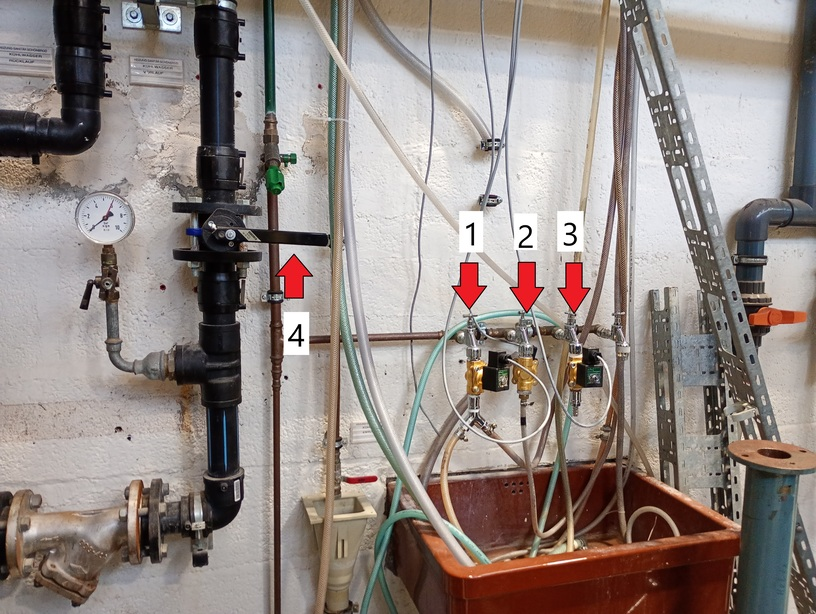
\includegraphics[width=\linewidth]{Cool2}
\end{figure}

\begin{enumerate}
	\item Cooling EC source and window
	\item Cooling turbopump
	\item Not in use
	\item Main valve Cooling for magnets
\end{enumerate}


\newpage
%%%%%%%%%%%%%%%%%%%%%%%%%%%%%%
\section{System preparation}%%	
%%%%%%%%%%%%%%%%%%%%%%%%%%%%%%

\begin{minipage}{.68\textwidth}
To operate the TOMAS device, several preparatory actions are necessary.

\subsection{The Operator PC} To operate the TOMAS device you have to login to the Operator PC (Figure \ref{PC1}). The username is \textit{'tomas'}. No password is required.\\

\changemenucolor{gray}{txt}{named}{red}
\textcolor{red}{\textbf{Press \keys{\ctrl + \Alt + \del} to get to the login screen. Press \keys{\enter} to login to the Operator PC. }}\\
\changemenucolor{gray}{txt}{named}{black}

\begin{minipage}{.5\textwidth}
\begin{tabular}{ll}
	PC name: &IPP126.ipp.kfa-juelich.de\\
	Username: &tomas\\
	Password: &(nopassword)
\end{tabular}
\end{minipage}
\begin{minipage}{.5\textwidth}
	\begin{tabular}{ll}
		IPv4 Address: &134.94.244.185\\
		Subnet Mask:& 255.255.252.0\\
		Default Gateway:& 134.94.244.1
	\end{tabular}
\end{minipage}
\vspace{0.6cm}

\begin{minipage}{.76\textwidth}
\subsubsection{Arduino operation} Open the 'Arduino IDE' app on the Operator PC. This will open automatically the code 'TOMASsteppers.ino' (Figure \ref{Arduino2}). At the bottom right you can verify on which COM-port the Arduino is located. Push the arrow button at the top left of the app to upload the sketch to the Arduino.\\

\textcolor{red}{\textbf{Open the 'Arduino IDE' app and upload the sketch 'TOMASsteppers.ino' to the Arduino.}}\\

\end{minipage}
\begin{minipage}{.02\textwidth}
$\ $\\
\end{minipage}
\begin{minipage}{.2\textwidth}
\centering

\includegraphics[width=\linewidth]{Arduino1}
\end{minipage}

\end{minipage}
\begin{minipage}{.02\textwidth}
$\ $\\
\end{minipage}
\begin{minipage}{.3\textwidth}
\centering
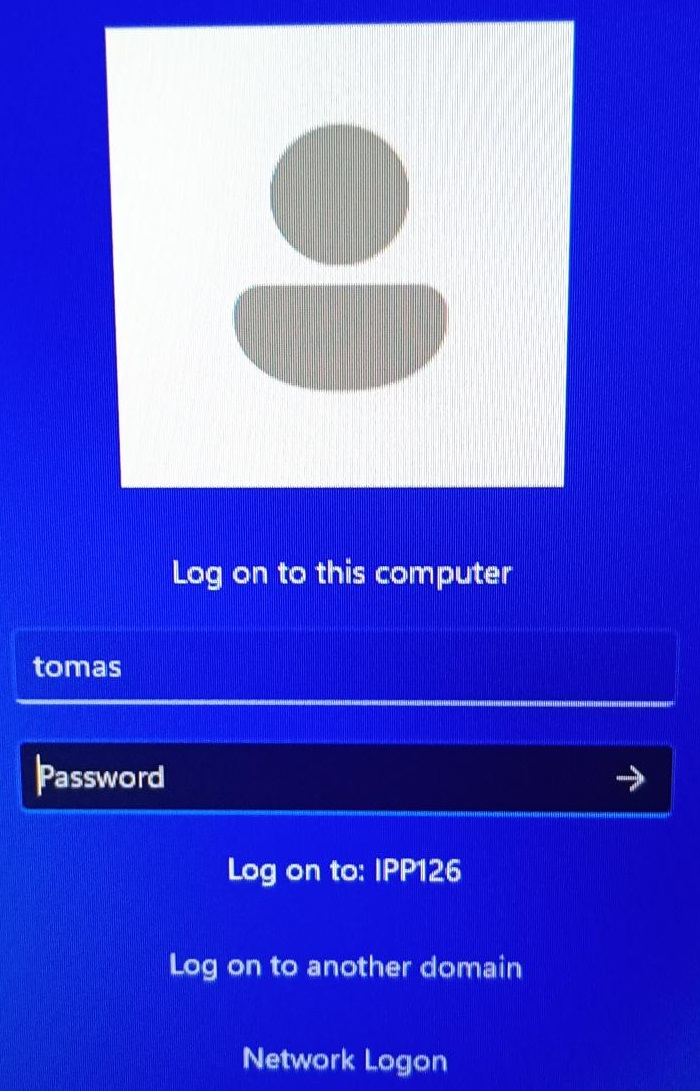
\includegraphics[width=\linewidth]{PC2}
\label{PC1}
\captionof{figure}{Operator PC Login screen}
\end{minipage}
%\vspace{0.2cm}

\begin{minipage}{\textwidth}
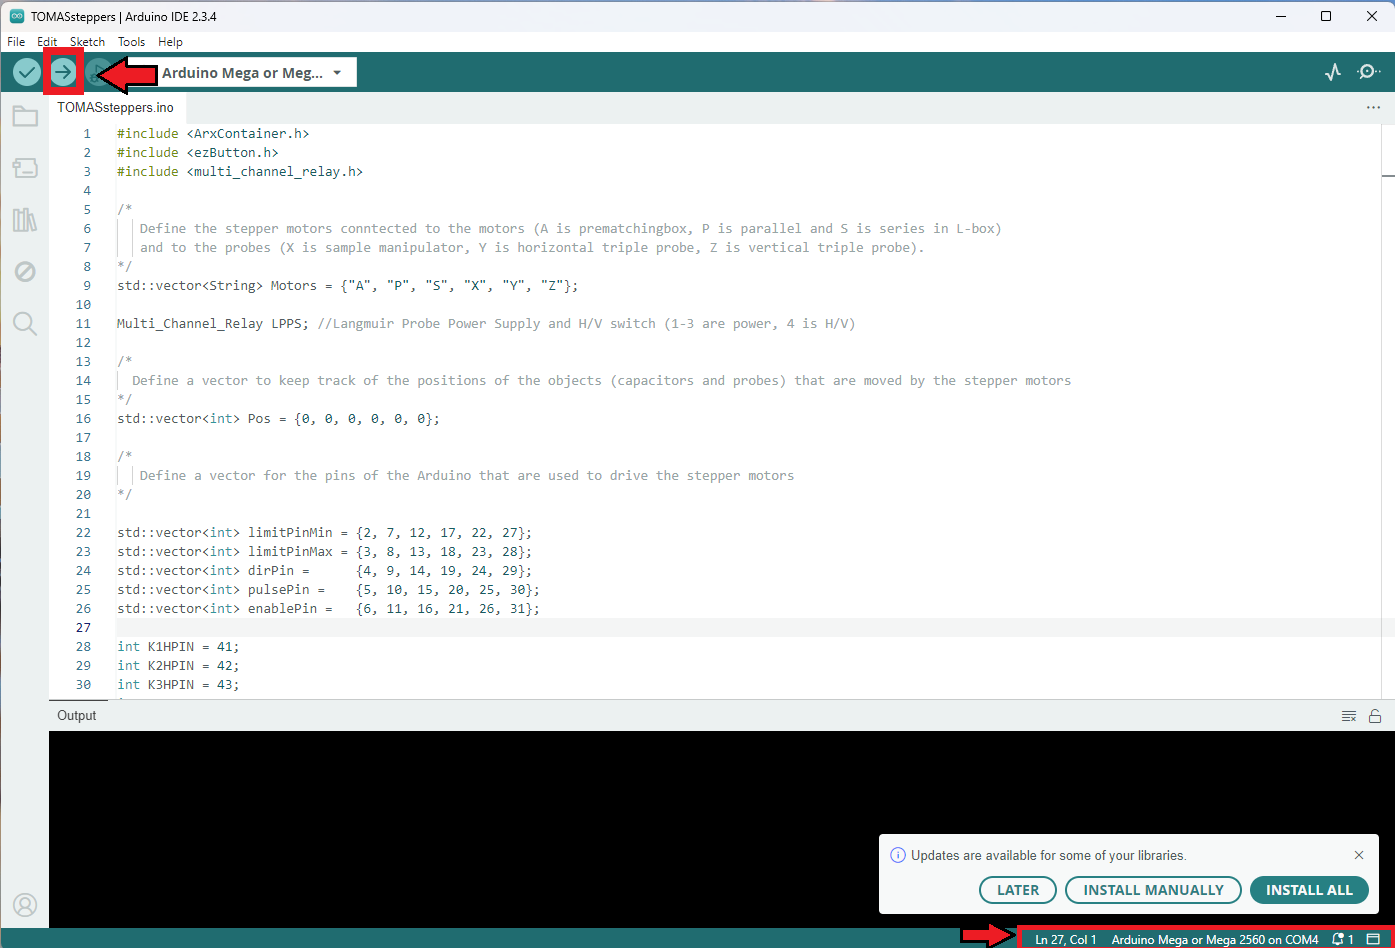
\includegraphics[width=\linewidth]{Arduino2}
\label{Arduino2}
\captionof{figure}{'Arduino IDE' app and 'TOMASsteppers.ino' sketch}
\end{minipage}

\newpage

\begin{minipage}{.83\textwidth}
\subsubsection{TOMAS Operation GUI}

Open the 'Spyder' app. This will automatically open several python scripts (Figure 	\ref{Spyder2}). Run the 'main.py' script by clicking the arrow button on the top left. This will open the TOMAS Operation GUI (Figure \ref{GUI1}). This Graphical User Interface controls several systems on TOMAS: the IC matching system, probe manipulation and the IC and EC power system. You can also introduce several System parameters which will be stored in a specific file for future reference.\\

\textcolor{red}{\textbf{Open the TOMAS Operation GUI.}}\\
\end{minipage}
\begin{minipage}{.02\textwidth}
$\ $\\
\end{minipage}
\begin{minipage}{.15\textwidth}
\centering

\includegraphics[width=0.85\linewidth]{Spyder1}
\end{minipage}

\begin{minipage}{\textwidth}
	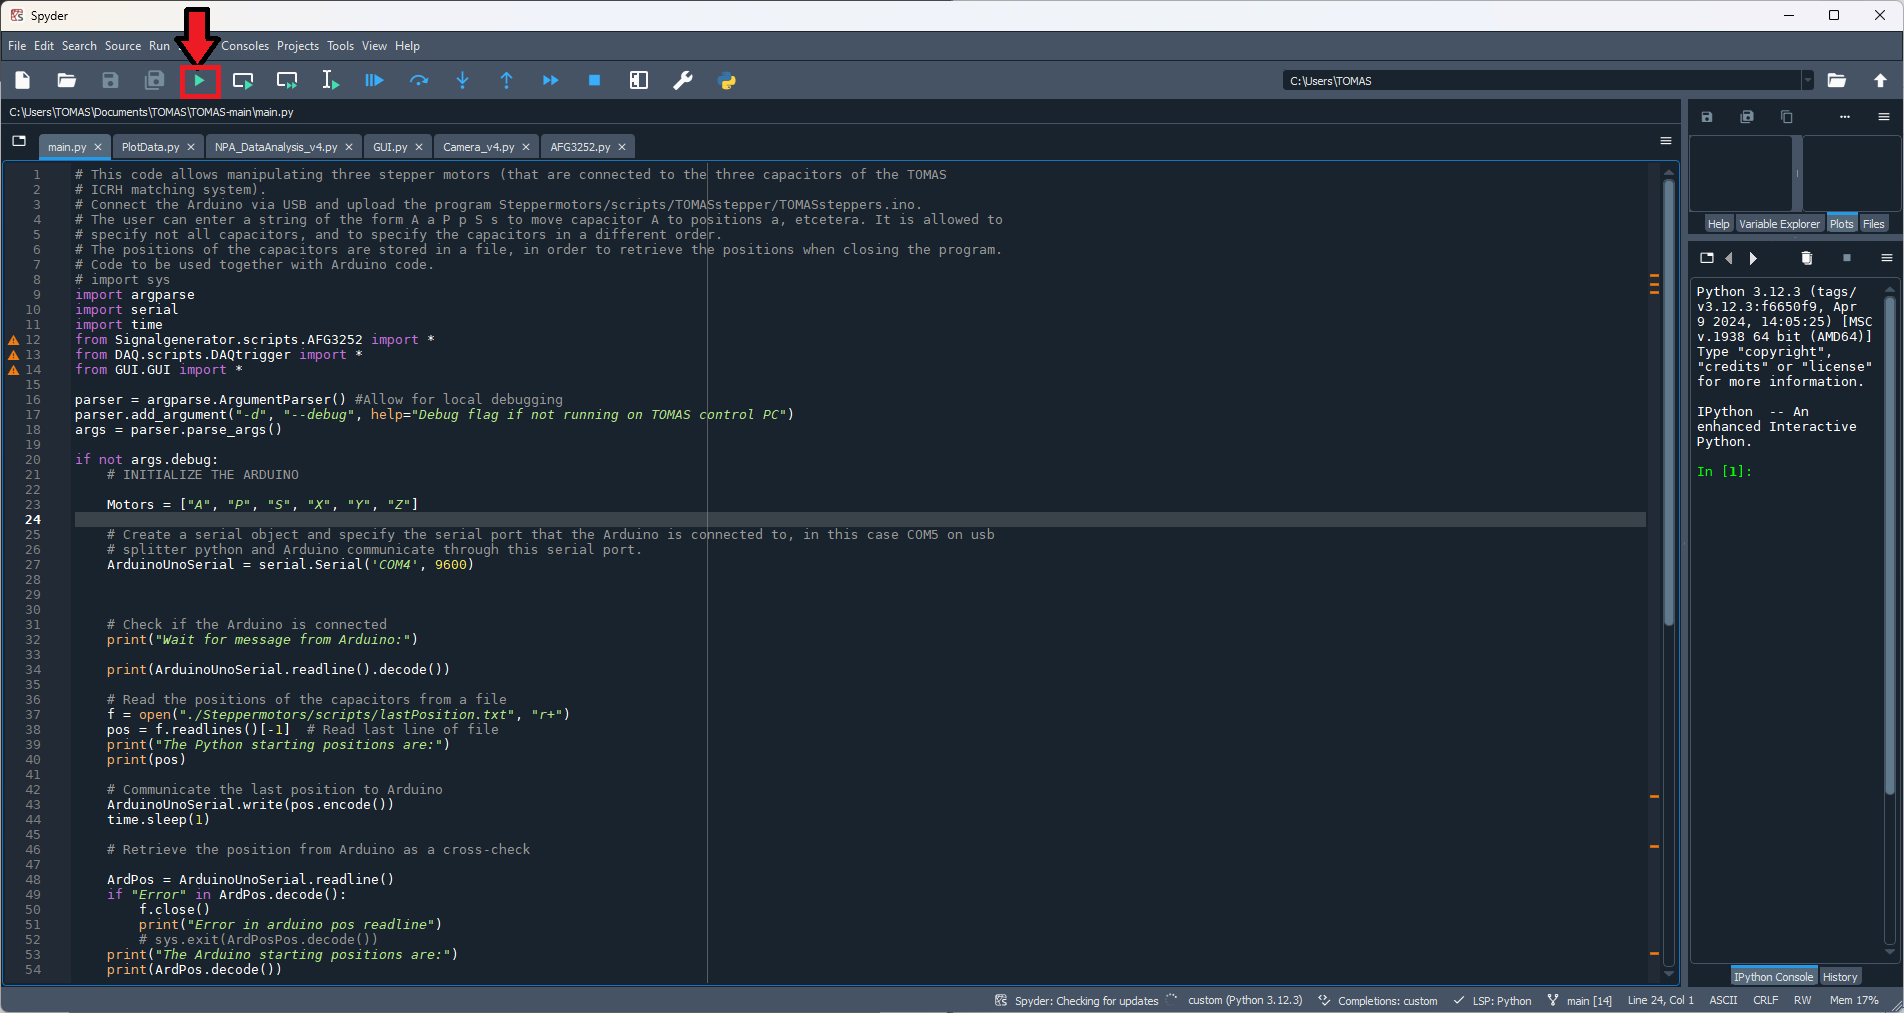
\includegraphics[width=\linewidth]{Spyder2}
	\label{Spyder2}
	\captionof{figure}{'Spyder' app and 'main.py' python script}
	\vspace{0.6cm}
	
	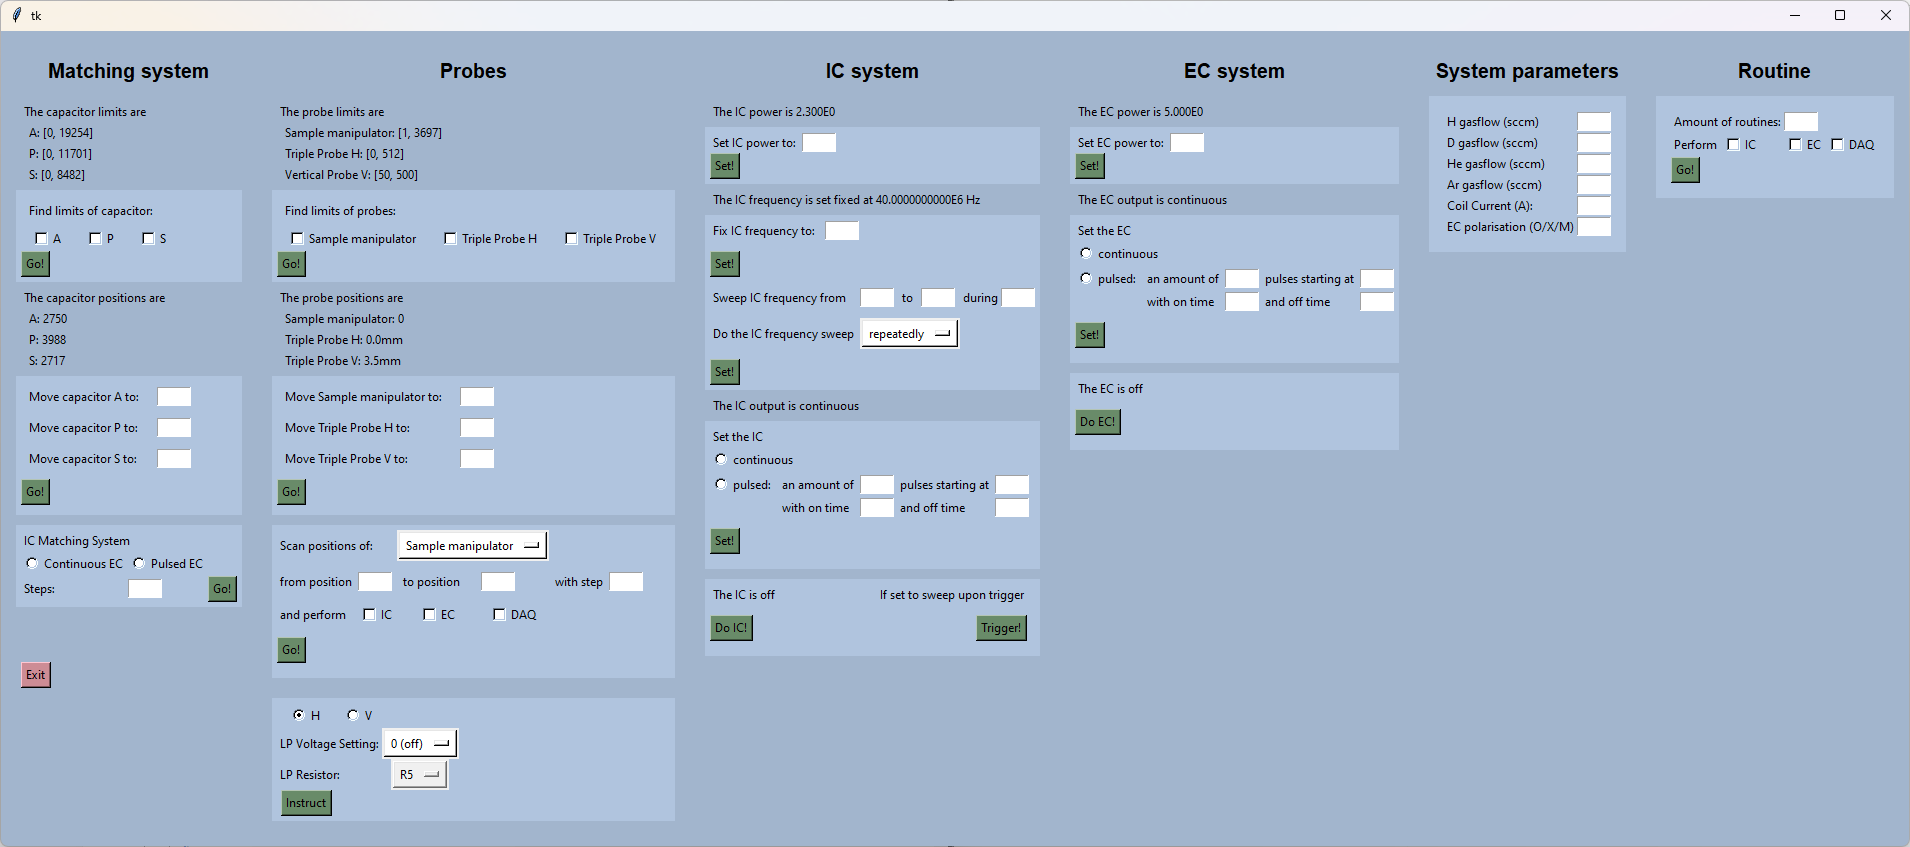
\includegraphics[width=\linewidth]{GUI1}
	\label{GUI1}
	\captionof{figure}{TOMAS Operation GUI}
\end{minipage}

\newpage
The TOMAS Operation GUI indicates the capacitor limits of the matching system, the probe position limits and the sample manipulator limits. It also indicates the actual positions of the capacitors, the probes and the sample manipulator.\\

\begin{minipage}{.5\textwidth}
The capacitor limits are:\\
A: [0, 19254]\\
P: [0, 11701]\\
S: [0, 8482]
\end{minipage}
\begin{minipage}{.5\textwidth}
The probe limits are:\\
Sample Manipulator: [1, 3697]\\
Horizontal Triple Probe: [0, 512]\\
Vertical Triple Probe: [50, 500]
\end{minipage}



\subsubsection{Camera Operation}

\begin{minipage}{.78\textwidth}
	Open the 'Camera' app on the Operator PC. It will normally by default open the 'B525 HD Webcam', which is located at the tangential port where the gas is injected.\\
	
	\textcolor{red}{\textbf{Open the 'Camera' app on the Operator PC.}}\\
	
In the future - when the new cameras are installed - a python script will be written to open and display the different video streams.
	
\end{minipage}
\begin{minipage}{.02\textwidth}
	$\ $\\
\end{minipage}
\begin{minipage}{.15\textwidth}
	\centering
	
\includegraphics[width=0.85\linewidth]{Cam1}
\end{minipage}


%\begin{minipage}{\textwidth}
%	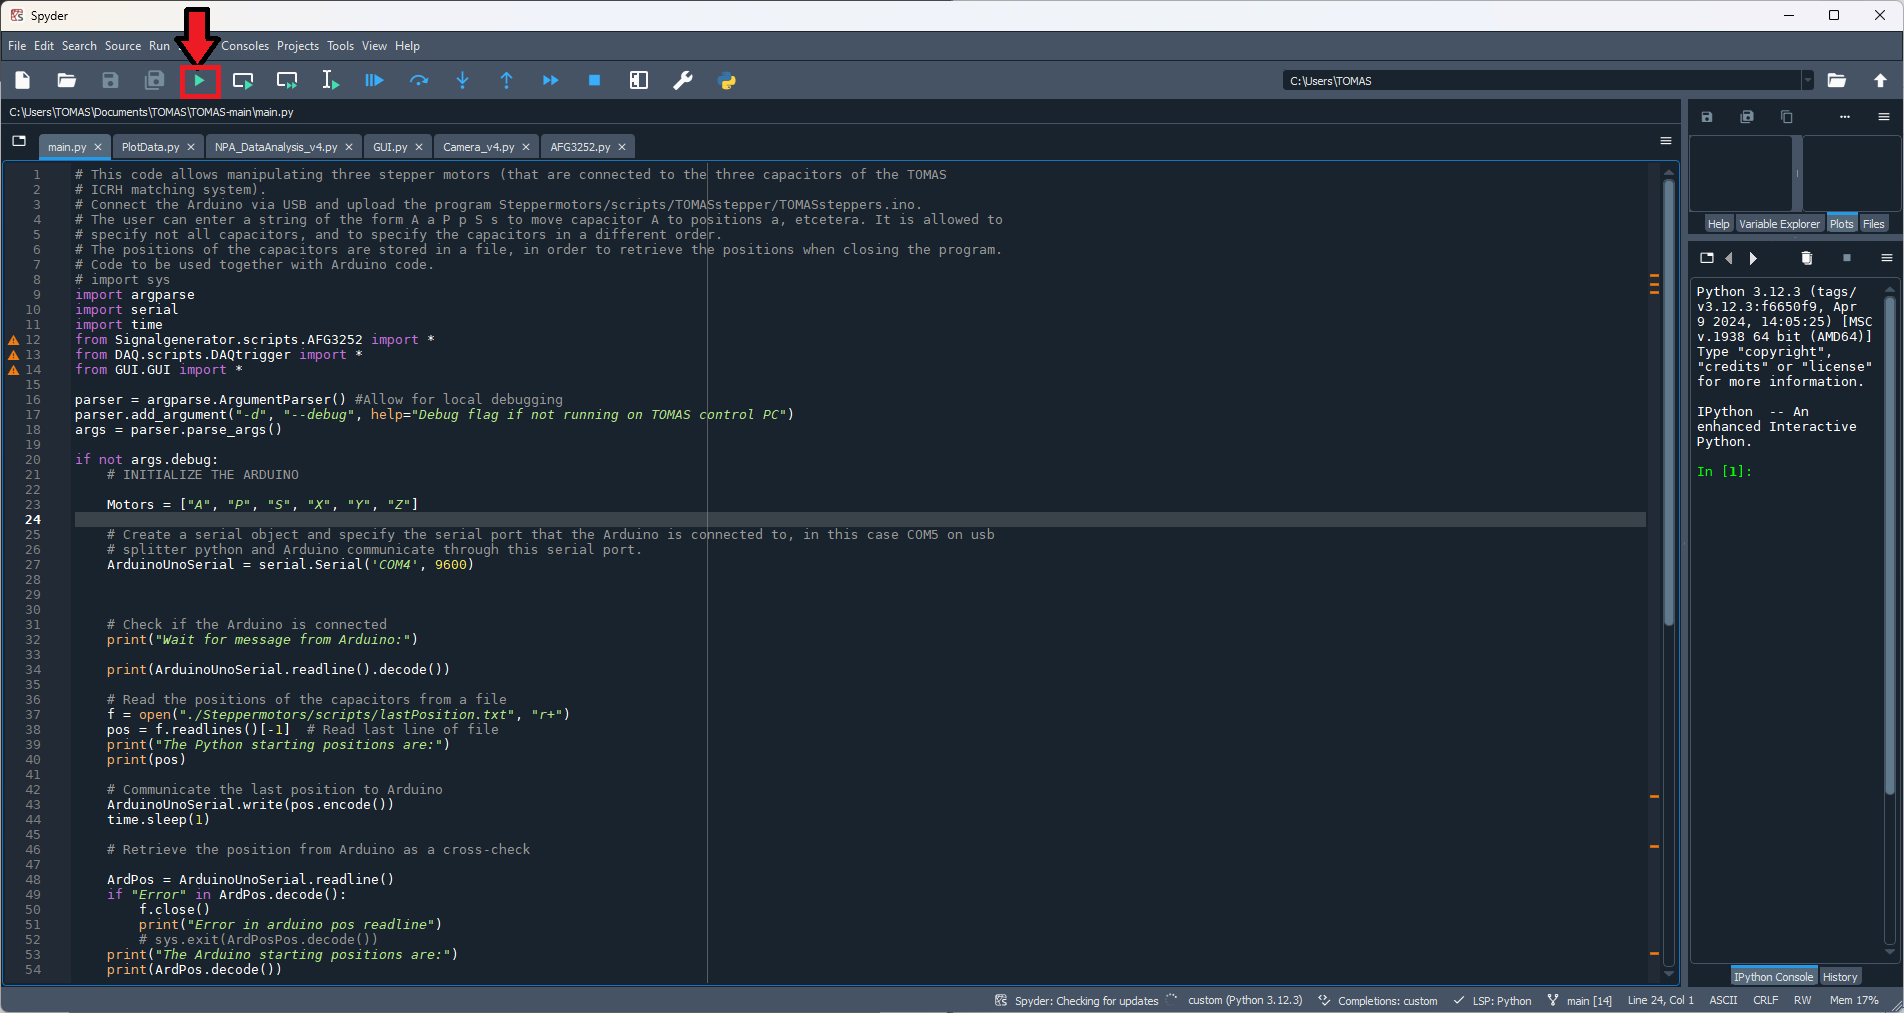
\includegraphics[width=\linewidth]{Spyder2}
%	\label{Spyder2}
%	\captionof{figure}{'Spyder' app and 'main.py' python script}
%\end{minipage}

\newpage
\subsection{The Control System}
\begin{minipage}{.78\textwidth}
To access the Control System, you can open a Remote Desktop connection on the Operator PC using the 'Remote Desktop' app. Click on the tile 'Control System' (Figure \ref{Remote2}).\\

\textcolor{red}{\textbf{Open a Remote Desktop connection to the Control System.}}\\

\begin{minipage}{.58\textwidth}
	\begin{tabular}{ll}
		PC name: & IPPTOMAS-WCC1.ipp.kfa-juelich.de\\
		Username: &CoDac\\
		Password: &ChL*2020
	\end{tabular}
\end{minipage}
\begin{minipage}{.42\textwidth}
	\begin{tabular}{ll}
		IPv4 Address: & xxx.xxx.xxx.xxx\\
		Subnet Mask:& xxx.xxx.xxx.xxx\\
		Default Gateway:& xxx.xxx.xxx.xxx
	\end{tabular}
\end{minipage}
\vspace{0.6cm}

\end{minipage}
\begin{minipage}{.02\textwidth}
$\ $\\
\end{minipage}
\begin{minipage}{.2\textwidth}
\centering

\includegraphics[width=0.85\linewidth]{Remote1}
\end{minipage}


The main page shows different tabs. These will be discussed further on in this manual.\\

\begin{minipage}{\textwidth}
	\centering
	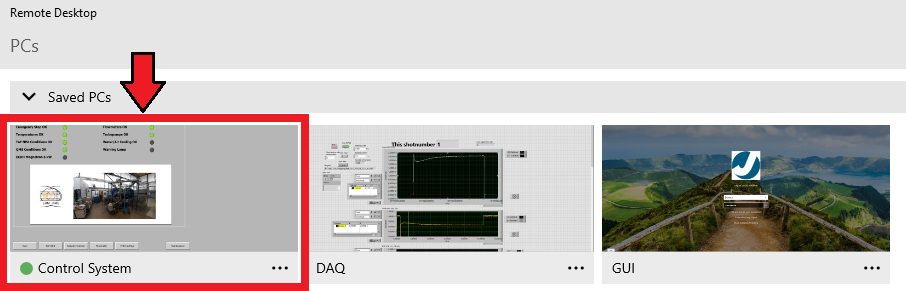
\includegraphics[width=\linewidth]{Remote2}
		\captionof{figure}{Remote Desktop connection to the Control System}
		\label{Remote2}
		\vspace{0.2cm}

	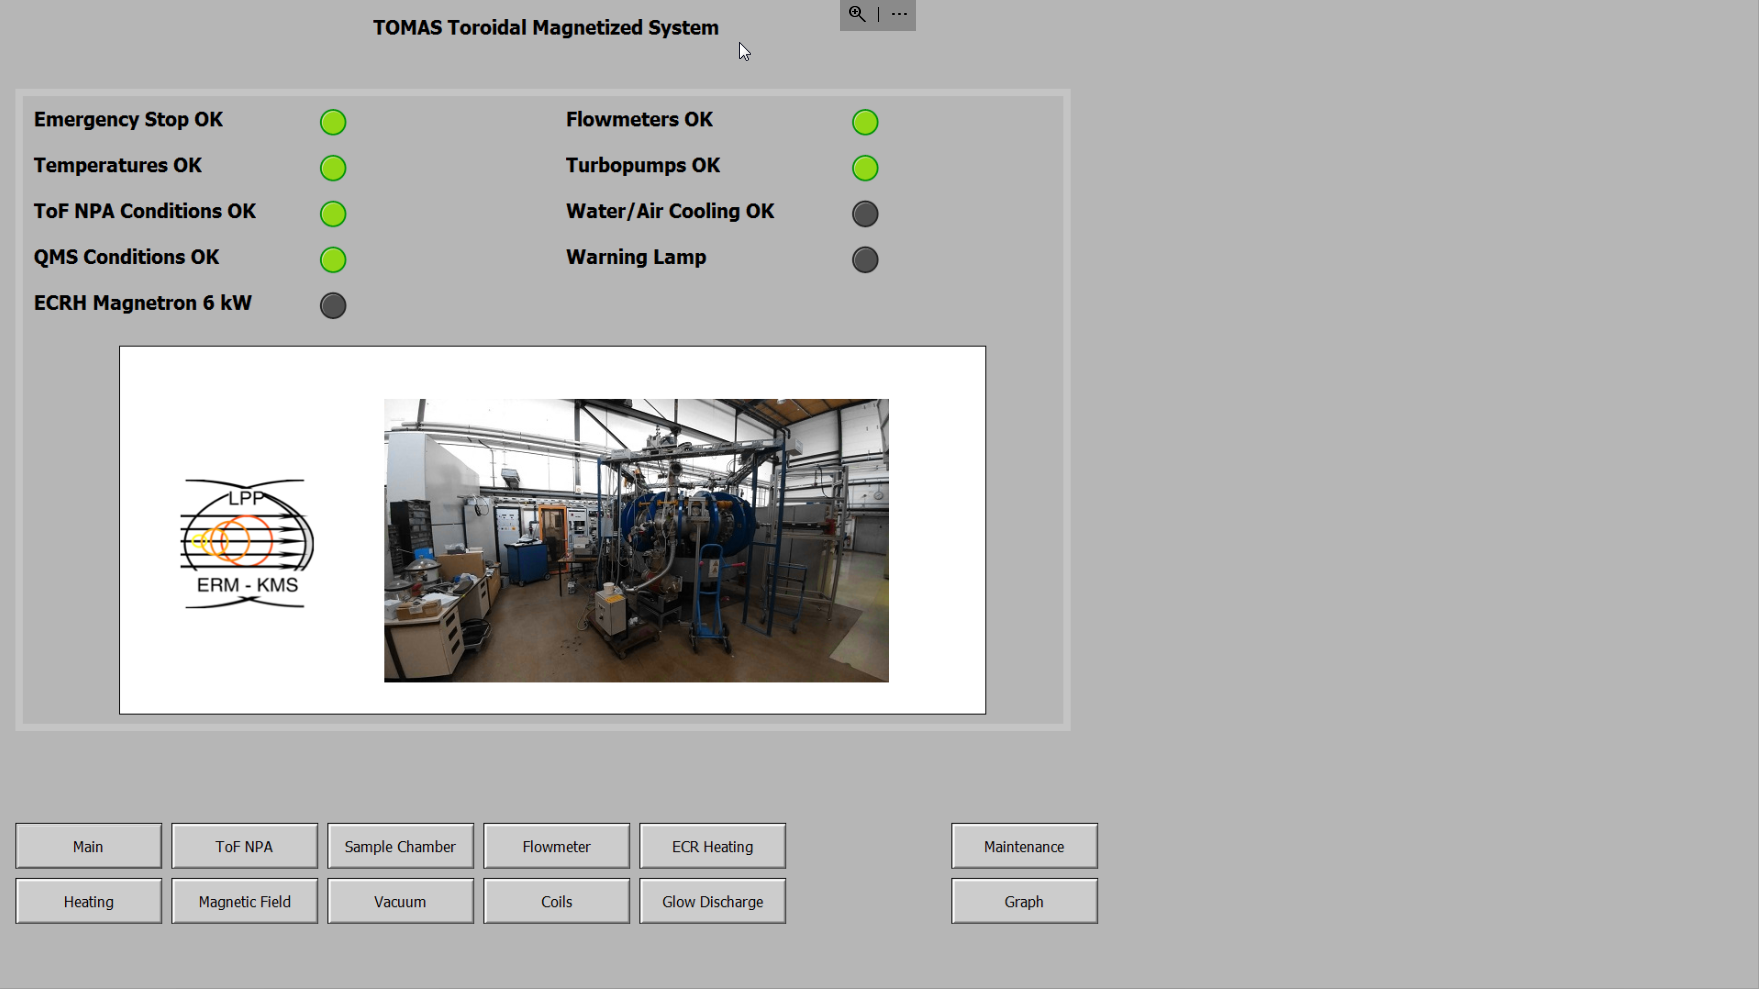
\includegraphics[width=\linewidth]{Remote3}
	\captionof{figure}{The Control System main page}
	\label{Remote3}
\end{minipage}



\newpage
\subsection{The Data Acquisition System}
\begin{minipage}{.78\textwidth}
	To access the Data Acquisition System, you can open a Remote Desktop connection on the Operator PC using the 'Remote Desktop' app. Click on the tile 'DAQ' (Figure \ref{Remote4}).\\
	
	\textcolor{red}{\textbf{Open a Remote Desktop connection to the  Data Acquisition System.}}\\
	
	\begin{minipage}{.58\textwidth}
		\begin{tabular}{ll}
			PC name: & IPP034.ipp.kfa-juelich.de\\
			Username: &Tecdaq\\
			Password: &TecdaqTEC
		\end{tabular}
	\end{minipage}
	\begin{minipage}{.42\textwidth}
		\begin{tabular}{ll}
			IPv4 Address: & 134.94.244.134\\
			Subnet Mask:& 255.255.252.0\\
			Default Gateway:& 134.94.244.134
		\end{tabular}
	\end{minipage}
	\vspace{0.6cm}
	
\end{minipage}
\begin{minipage}{.02\textwidth}
	$\ $\\
\end{minipage}
\begin{minipage}{.2\textwidth}
	\centering
	
\includegraphics[width=0.85\linewidth]{Remote1}
\end{minipage}

When you connect to the Data Acquisition System, you will notice that the LabVIEW file 'DAQ\_TOMAS\_AA.vi' is already loaded (Figure 	\ref{Remote5}), together with the Block Diagram. If not, open 'NI labVIEW2019 SP1 (32-bit)' and load the file 'DAQ\_TOMAS\_AA.vi'. The icon is on the DAQ Desktop.\\


To initialize the Data Acquisition, introduce the Sampling rate (default value: 1000 Hz), the Sampling time (default value: 12 s) and the Gas Type (H,D,He,Ar). Also introduce the starting value for the shot number (Start session with shotnumber : 1). Start the Data Acquisition by clicking the arrow on the top left. Enable data saving when required by clicking on 'Disabled'. The Data Acquisition System is now ready to receive the data.\\

\begin{minipage}{\textwidth}
	\centering
	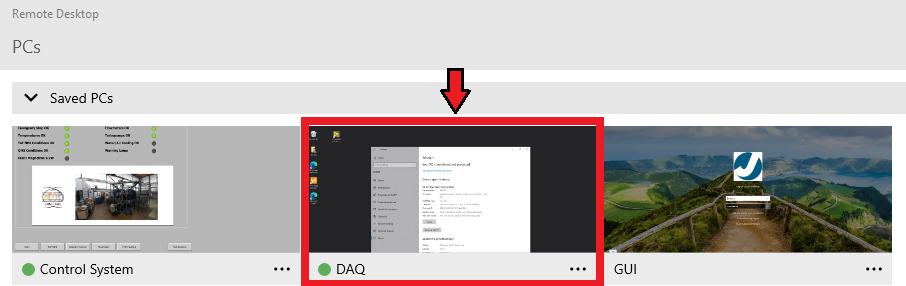
\includegraphics[width=\linewidth]{Remote4}
	\captionof{figure}{Remote Desktop connection to the Data Acquisition System}
	\label{Remote4}
	\vspace{0.2cm}
	
	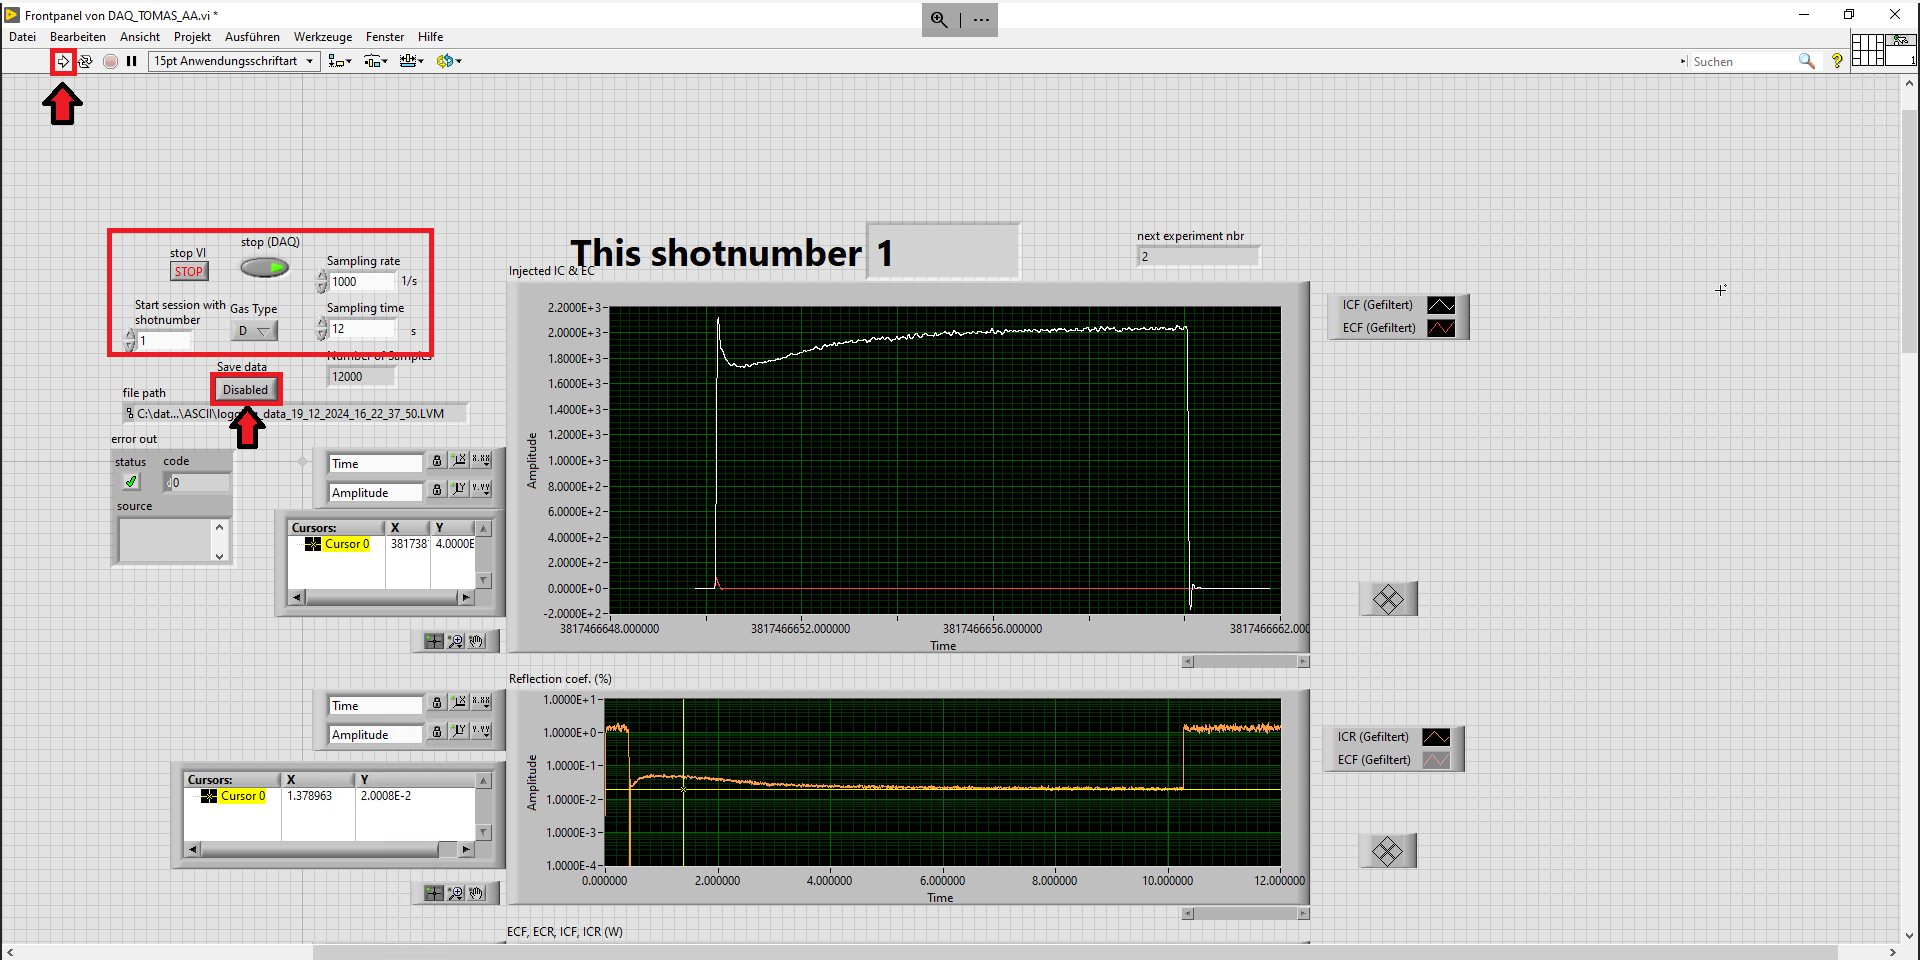
\includegraphics[width=\linewidth]{Remote5}
	\captionof{figure}{The LabVIEW file 'NI labVIEW2019 SP1 (32-bit)' on the Data Acquisition System}
	\label{Remote5}
\end{minipage}


\newpage








\begin{minipage}{.68\textwidth}
	
\subsection{The Vacuum and gas injection system}

The average neutral pressure is shown on the readout unit located in the main equipment rack.	The vacuum vessel pressure is shown on the Channel 1 (upper number) of the readout. To start an operation the pressure level should be $< 5\cdot 10^{-7}$ mbar. If the pressure is slightly higher check that calibration of the Channel 1 is set for N2 (air). In other cases, check the Troubleshooting.\\

\textcolor{red}{\textbf{Before starting any plasma operation, check the pressure in the vacuum vessel.}}\\

The gas injection system is located in a large support structure close to one of the tangential ports of the vacuum vessel. The gas injection system has 4 mass flow controllers directly connected to helium, hydrogen, argon and deuterium bottles.\\

\textcolor{red}{\textbf{Check that the gas bottles are closed.}}\\

The upstream and downstream pipes of the gas injection system must be evacuated from the residual gas prior an injection start.\\

Find the small metallic valves below the mass flow controllers (Figure \ref{Gas1} (1)). If any element above a valve is missing don’t open a corresponding valve! \\

\end{minipage}
\begin{minipage}{.02\textwidth}
	$\ $\\
\end{minipage}
\begin{minipage}{.3\textwidth}
	\centering
	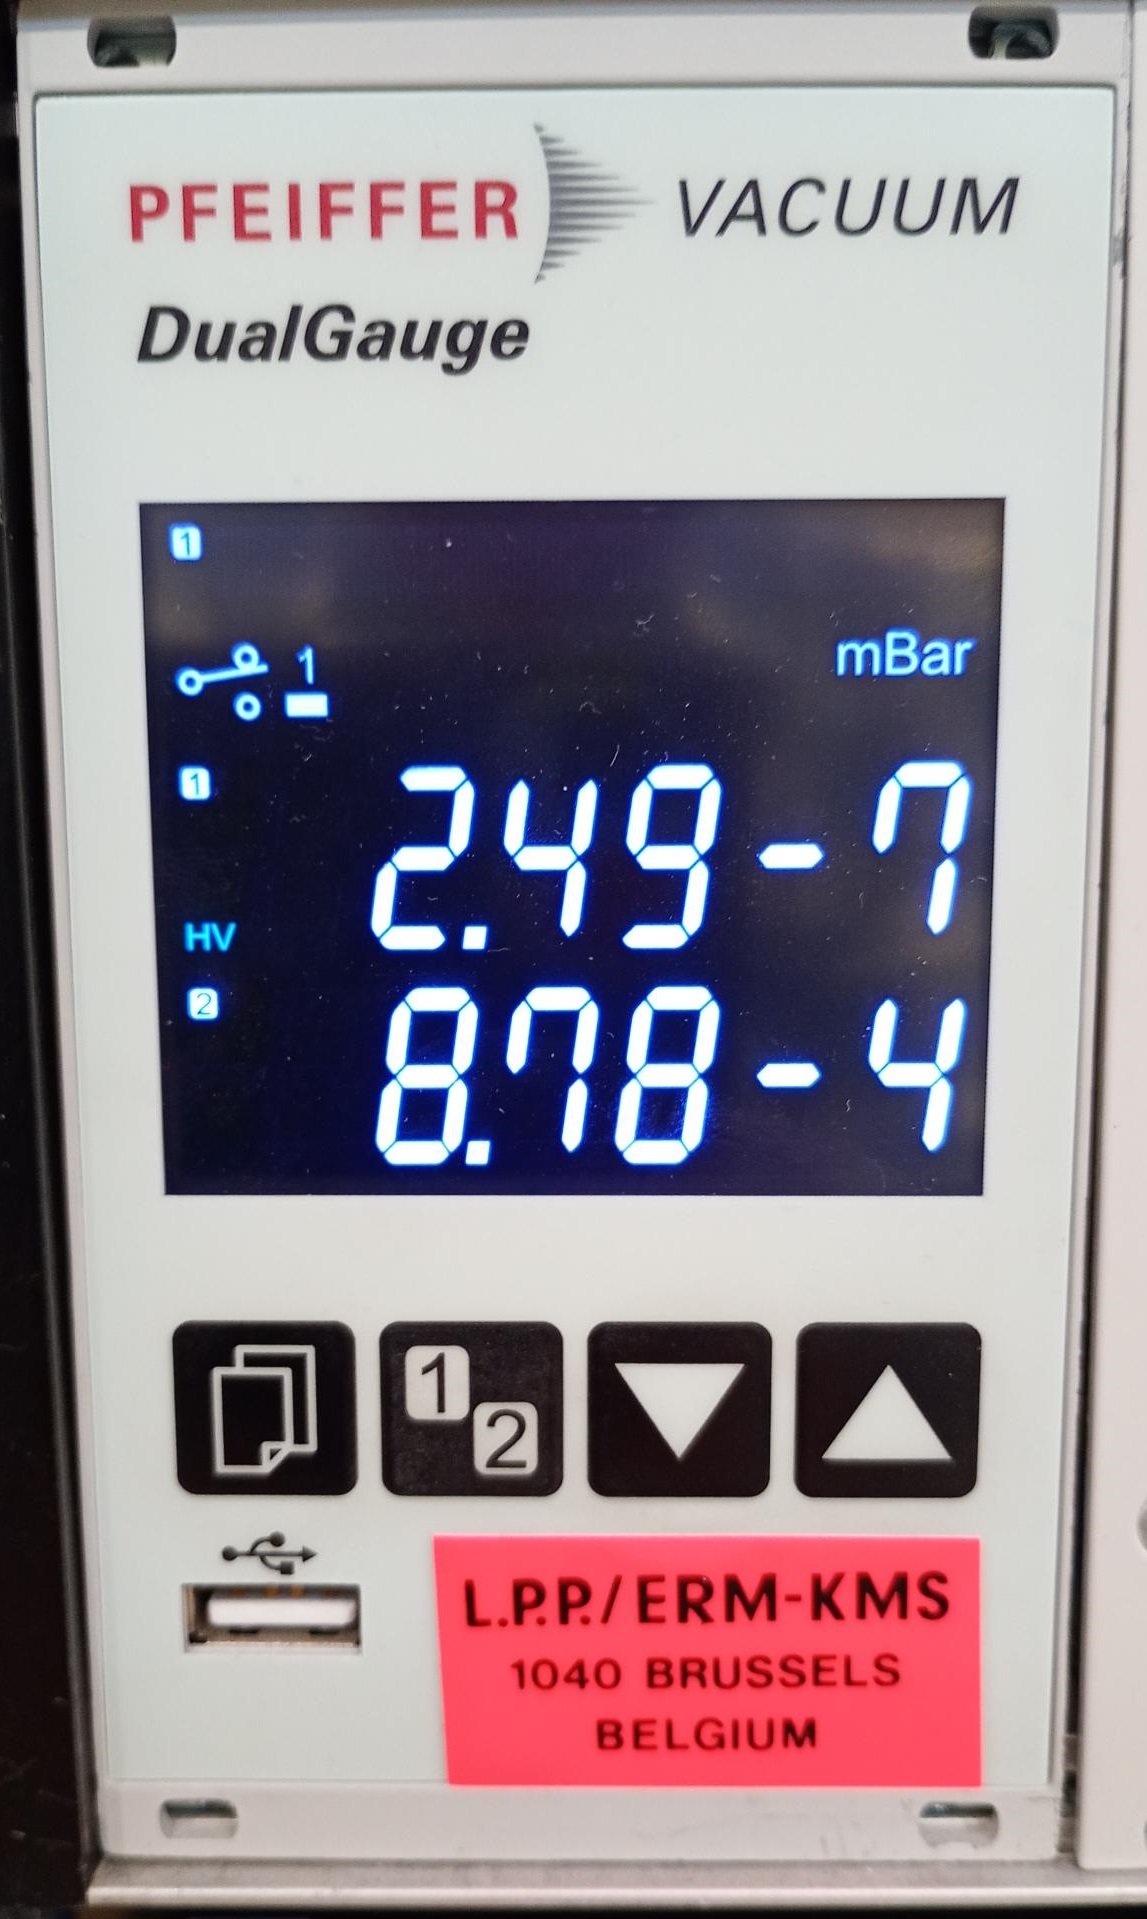
\includegraphics[width=\linewidth]{Pressure2}
\end{minipage}


\vspace{0.5cm}


\textcolor{red}{\textbf{Open the small metallic valves located below each mass flow controller (Figure \ref{Gas1} (1)).}}\\

Open the `\textit{Flowmeter}' tab in the Control System and go to the section \textbf{Pressure Control} the activate the `\textit{Forpump Flowmeter}' (Figure \ref{Gas2}).\\


\textcolor{red}{\textbf{Activate the Forepump to clear the lines (Figure \ref{Gas2}).}}\\


\begin{minipage}{.3\textwidth}
	
{Check if the vacuum pump connected to the upstream pipes is switched on. Pump down the upstream pipes during 10 – 15 minutes. }\\

{
	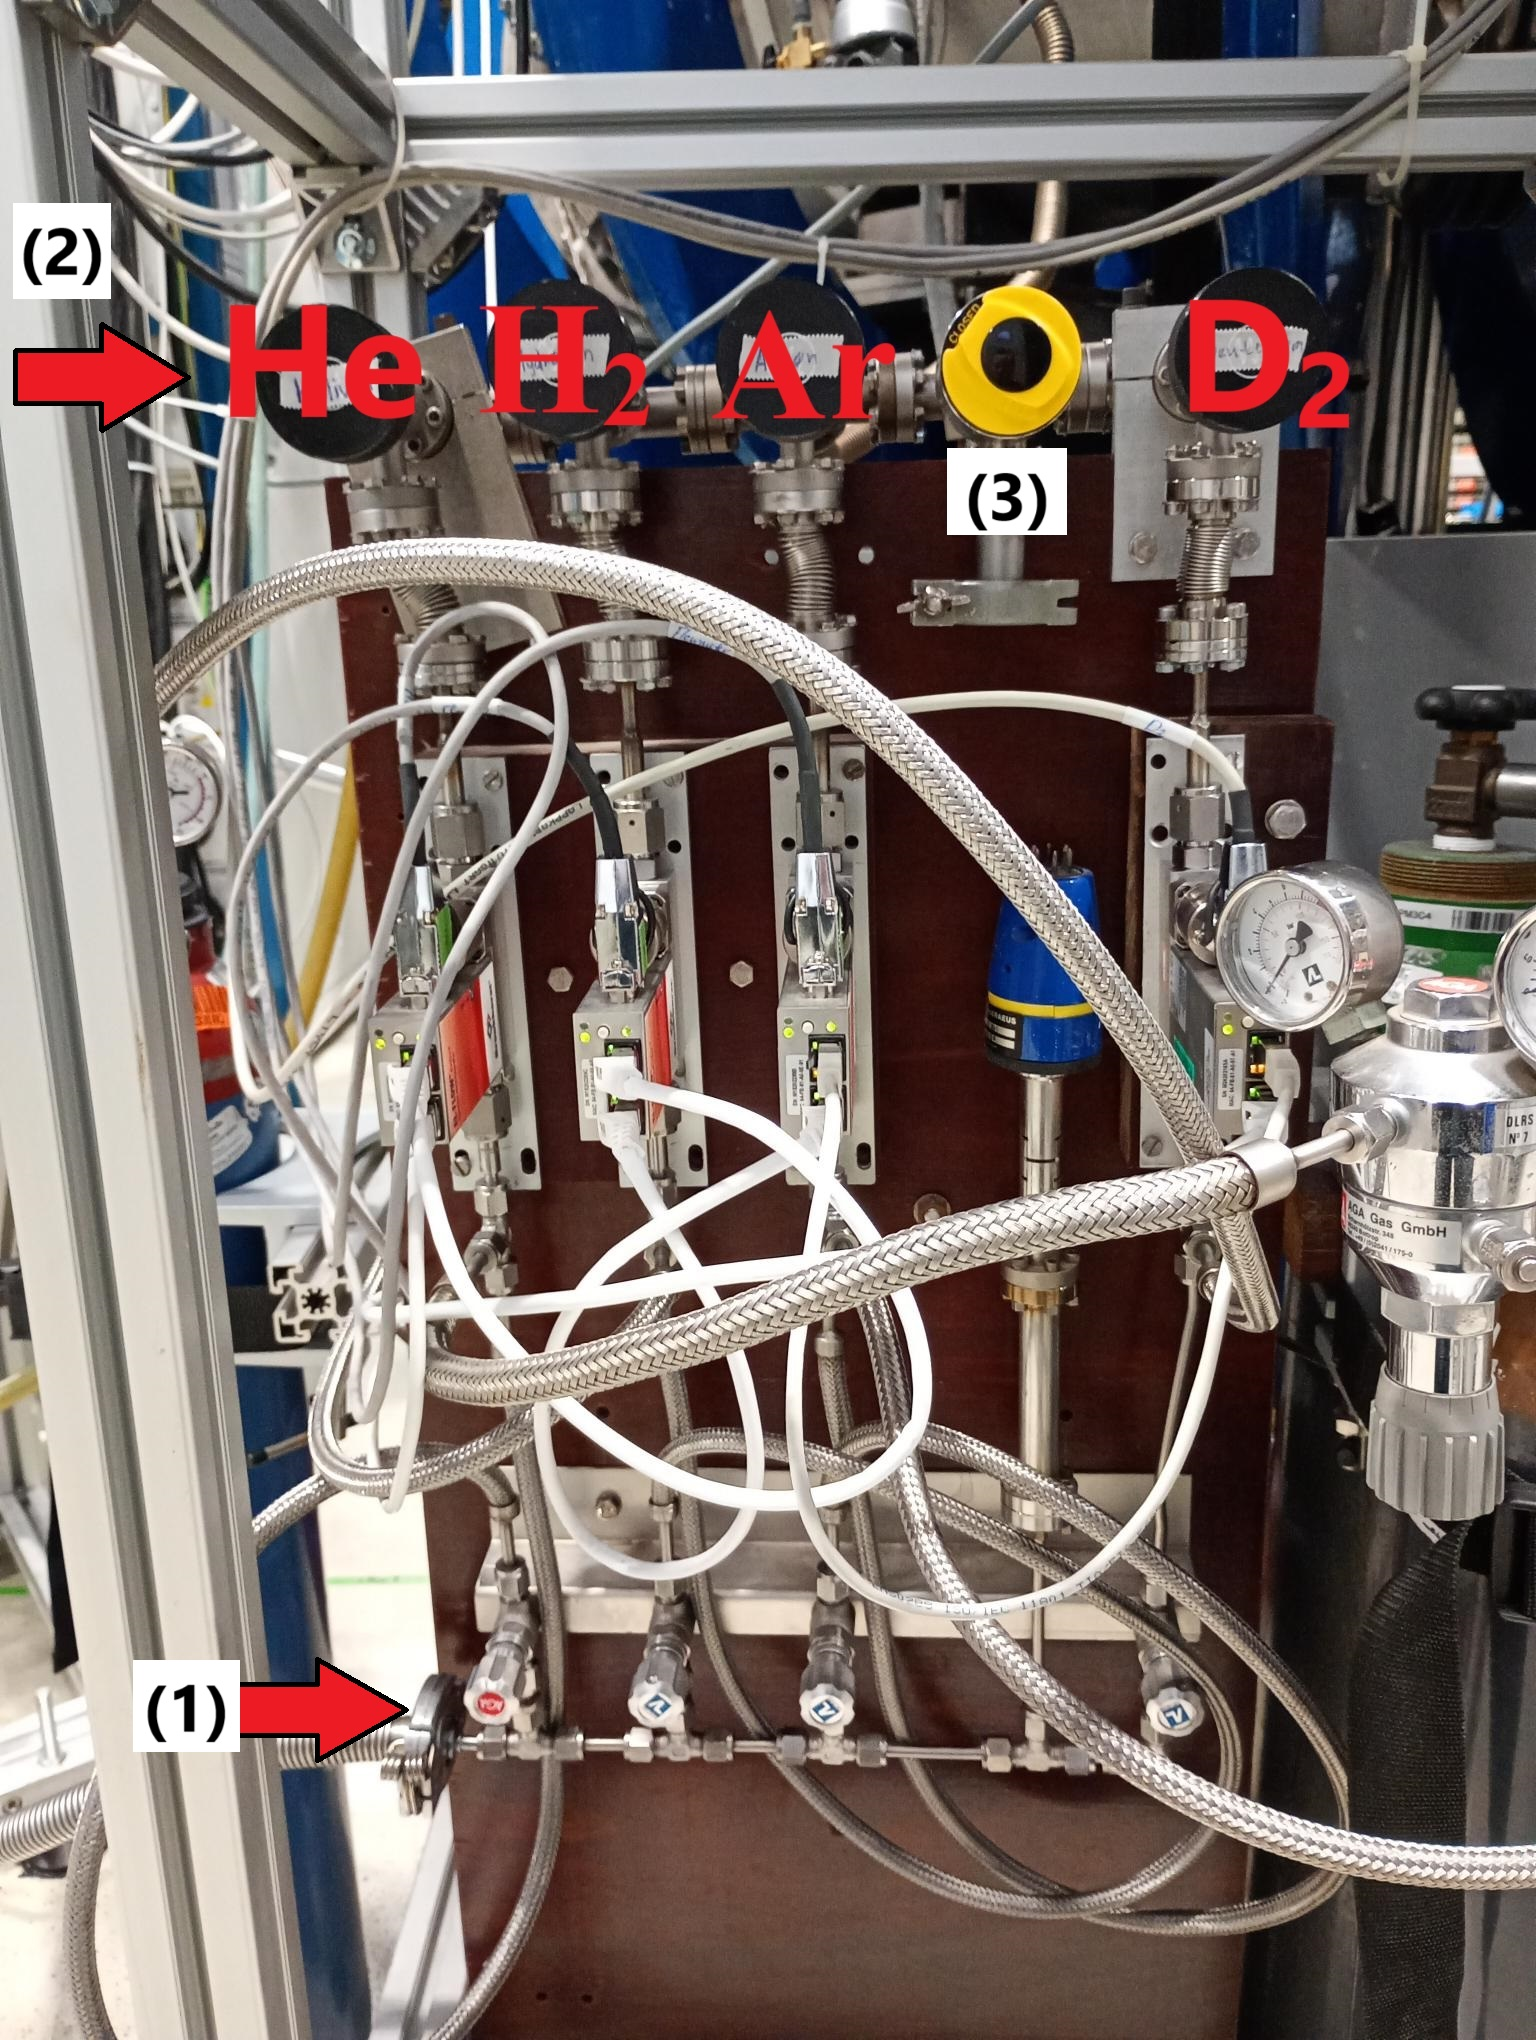
\includegraphics[width=\linewidth]{Gas1}
	\captionof{figure}{The gas injection system}
	\label{Gas1}}
\end{minipage}
\begin{minipage}{.02\textwidth}
	$\ $\\
\end{minipage}
\begin{minipage}{.68\textwidth}
	\centering
	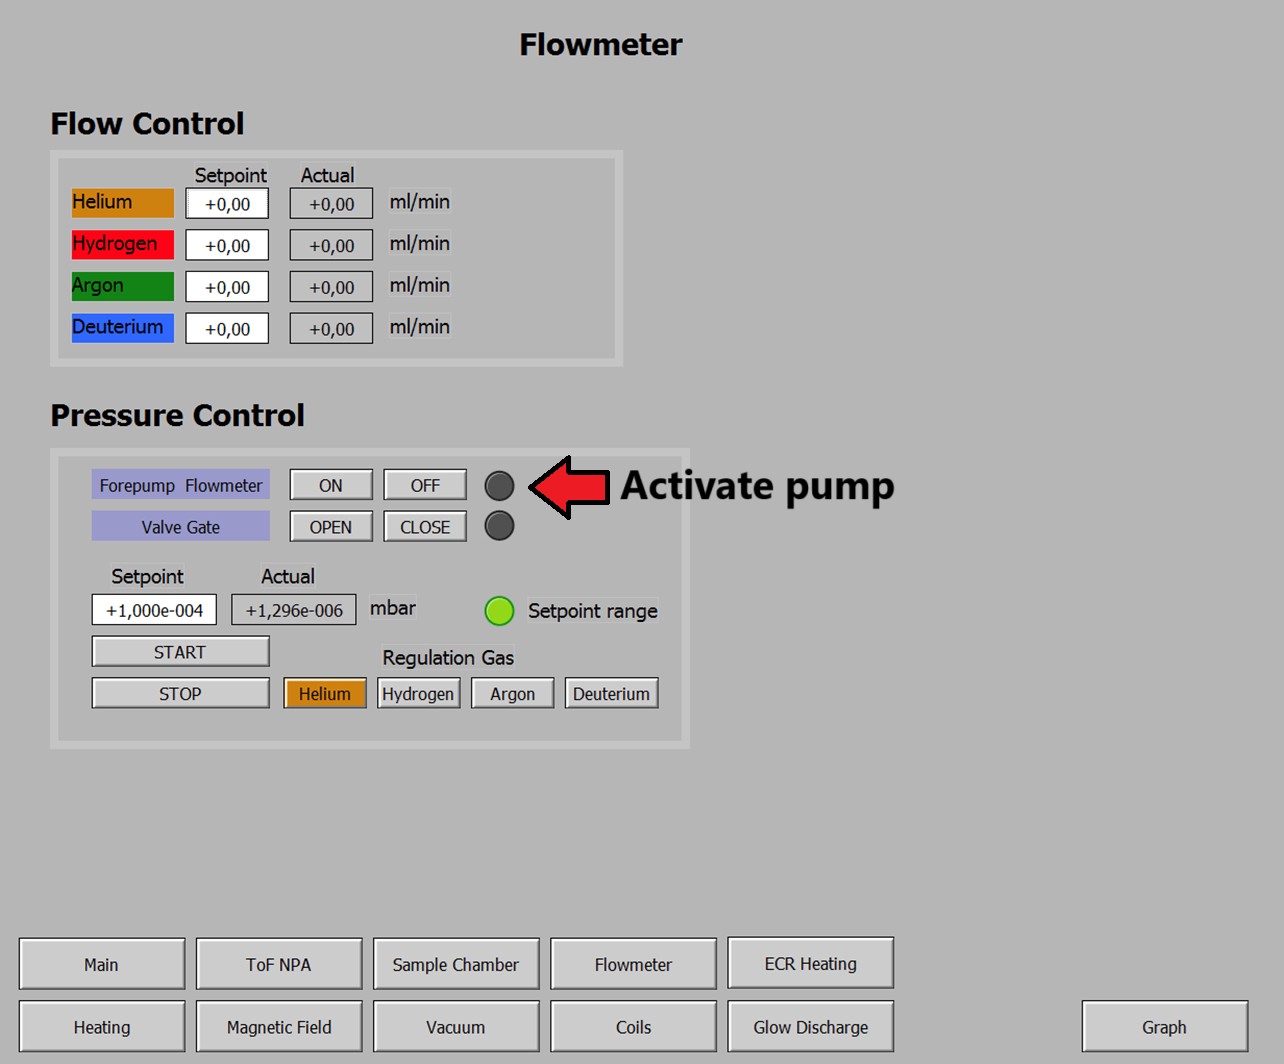
\includegraphics[width=0.95\linewidth]{Gas2}
	\captionof{figure}{The `\textit{Flowmeter}' tab in the Control System}
	\label{Gas2}
 
\end{minipage}	
\vspace{0.2cm}
	
\textcolor{red}{\textbf{Close all small metallic valves and deactivate the Forepump.}}\\

The gas injection system is now ready for operation.

\newpage

\begin{minipage}{.68\textwidth}

		
\textcolor{red}{\textbf{Open the needed bottle(s).}}\\

Check that both manometers on the gas reducer connected to each bottle shows a pressure different from 0. Otherwise, check the Troubleshooting.\\

\textcolor{red}{\textbf{Open the respective black valves above the mass flow controller(s) (Figure \ref{Gas1} (2)).}}\\


Don’t open the yellow valve (Figure \ref{Gas1} (3)). This is used to vent the machine. Check that the black shutter (Figure \ref{Gas3}) connecting the gas injection system to the tangential port is open (downward position). Since no gas is injected yet, the pressure level should not change significantly. If needed, wait until the pressure level is back below  $\approx 5\cdot 10^{-7}$ mbar.\\

The gas injection system is now ready for operation. Gas can be injected by the control system in the section \textit{`Flow Control'} in the \textit{`Flowmeter'} tab. Type the desired amount in the column \textit{`Setpoint'}. The actual injected amount is shown in the second column.\\

The minimum amount of gas is 10 ml/min for helium, hydrogen and argon. For deuterium the starting value should not be below 15 ml/min. You can decrease it afterwards to a minimum of 11 ml/min. 
\end{minipage}
\begin{minipage}{.02\textwidth}
$\ $\\
\end{minipage}
\begin{minipage}{.3\textwidth}
	\centering
	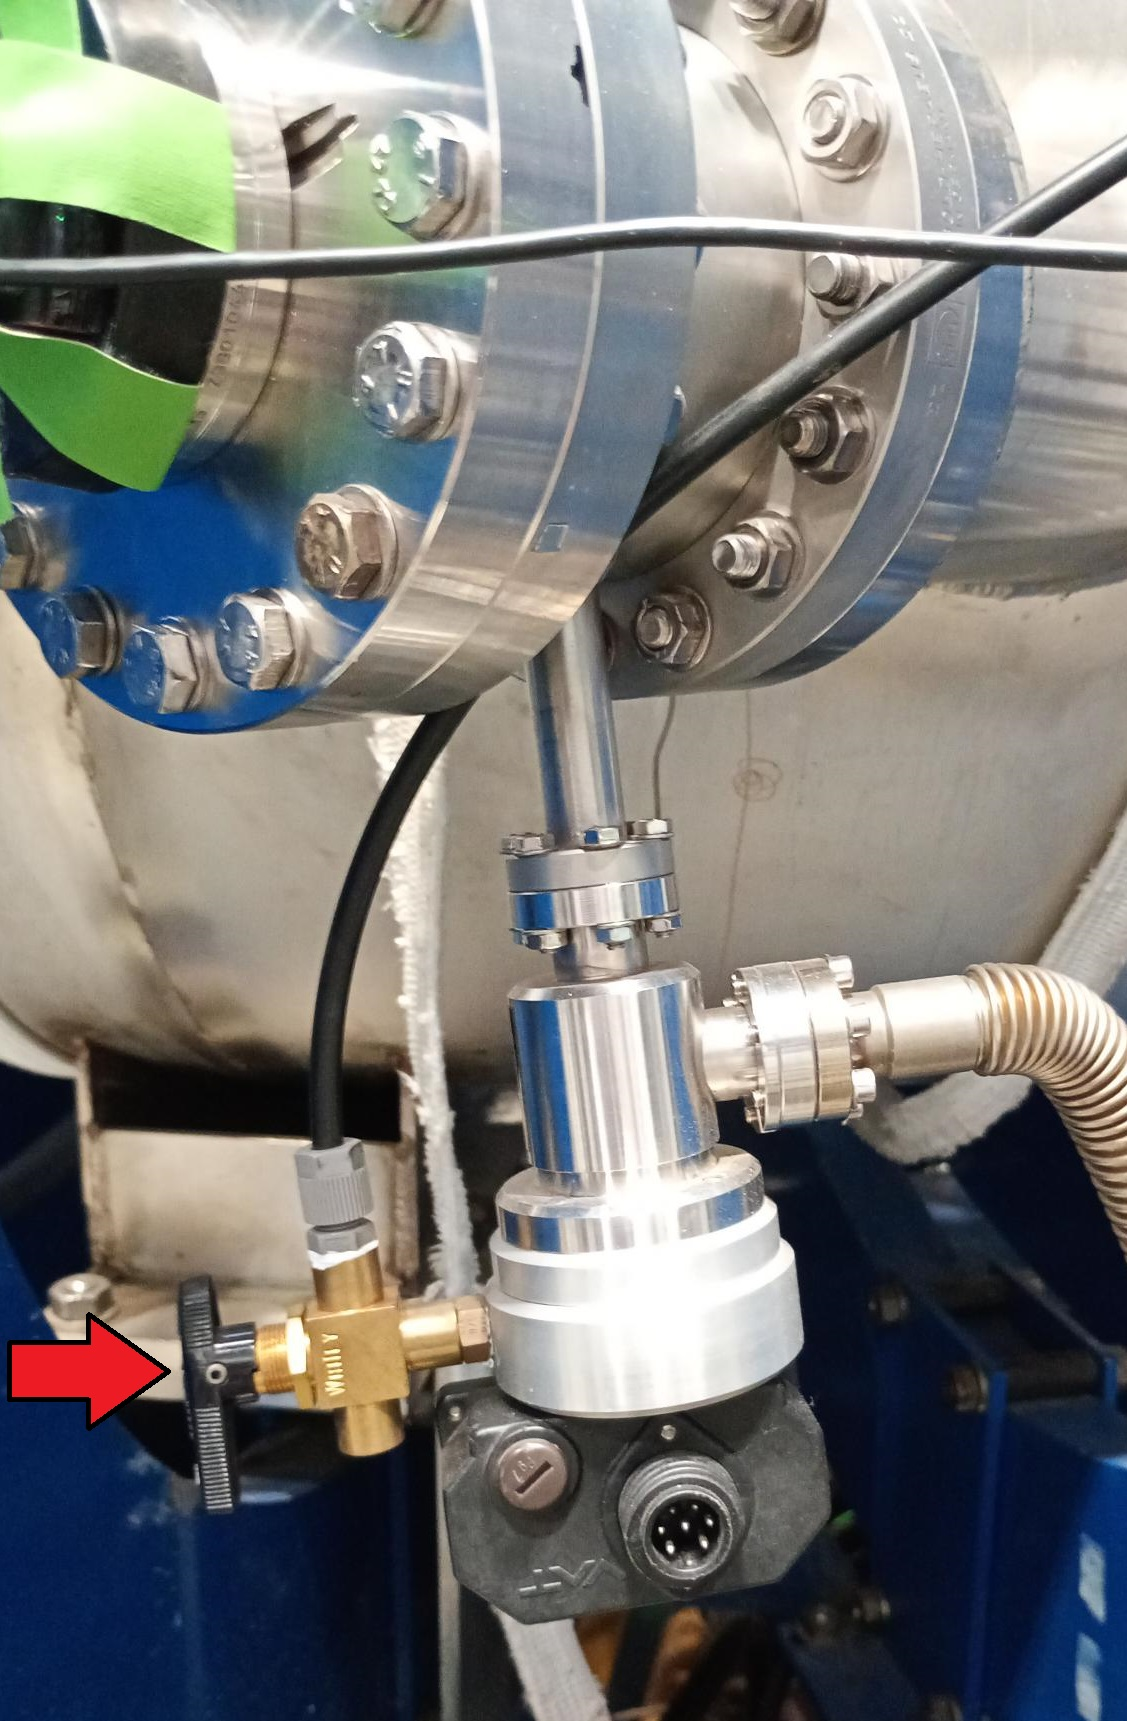
\includegraphics[width=\linewidth]{Gas3}
	\captionof{figure}{Shutter of the gas injection system}
	\label{Gas3}
\end{minipage}	
			

\subsection{Cooling}

The cooling system for the turbo-pump, the EC source and the EC window is activated automatically by the control system. The cooling system for the cooling of the coils has to be activated manually. This requires to change the position of the black lever arm from horizontal to $30^\circ$ (Figure \ref{Cool2} right). Position changing requires pushing the lever arm interlock.\\

\textcolor{red}{\textbf{Change the position of the black lever arm from horizontal to $30^\circ$ (Figure \ref{Cool2} right).}}\\

\textcolor{red}{\textbf{Verify that the water pump for the closed water circuit is activated (black button on Figure \ref{Cool9}).}}\\

\begin{figure}[!h]
	\centering
	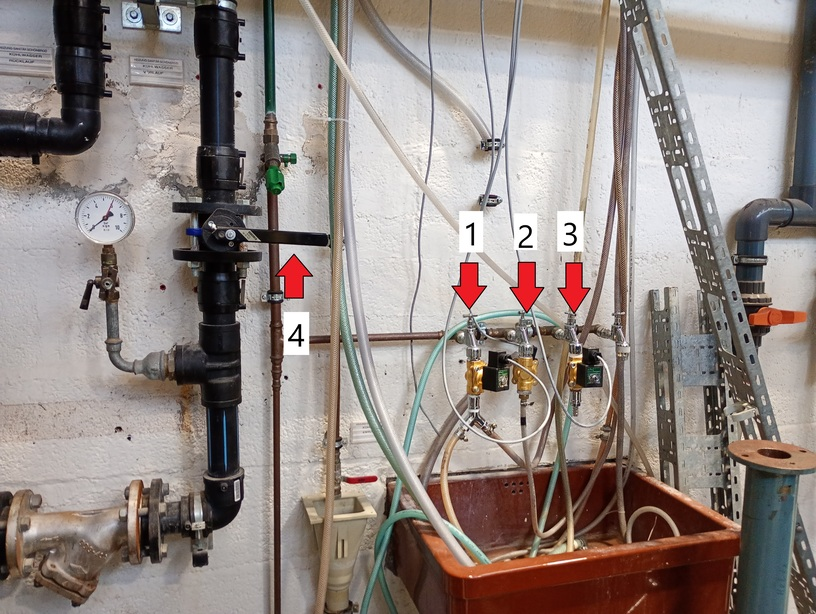
\includegraphics[height=8cm]{Cool2}
	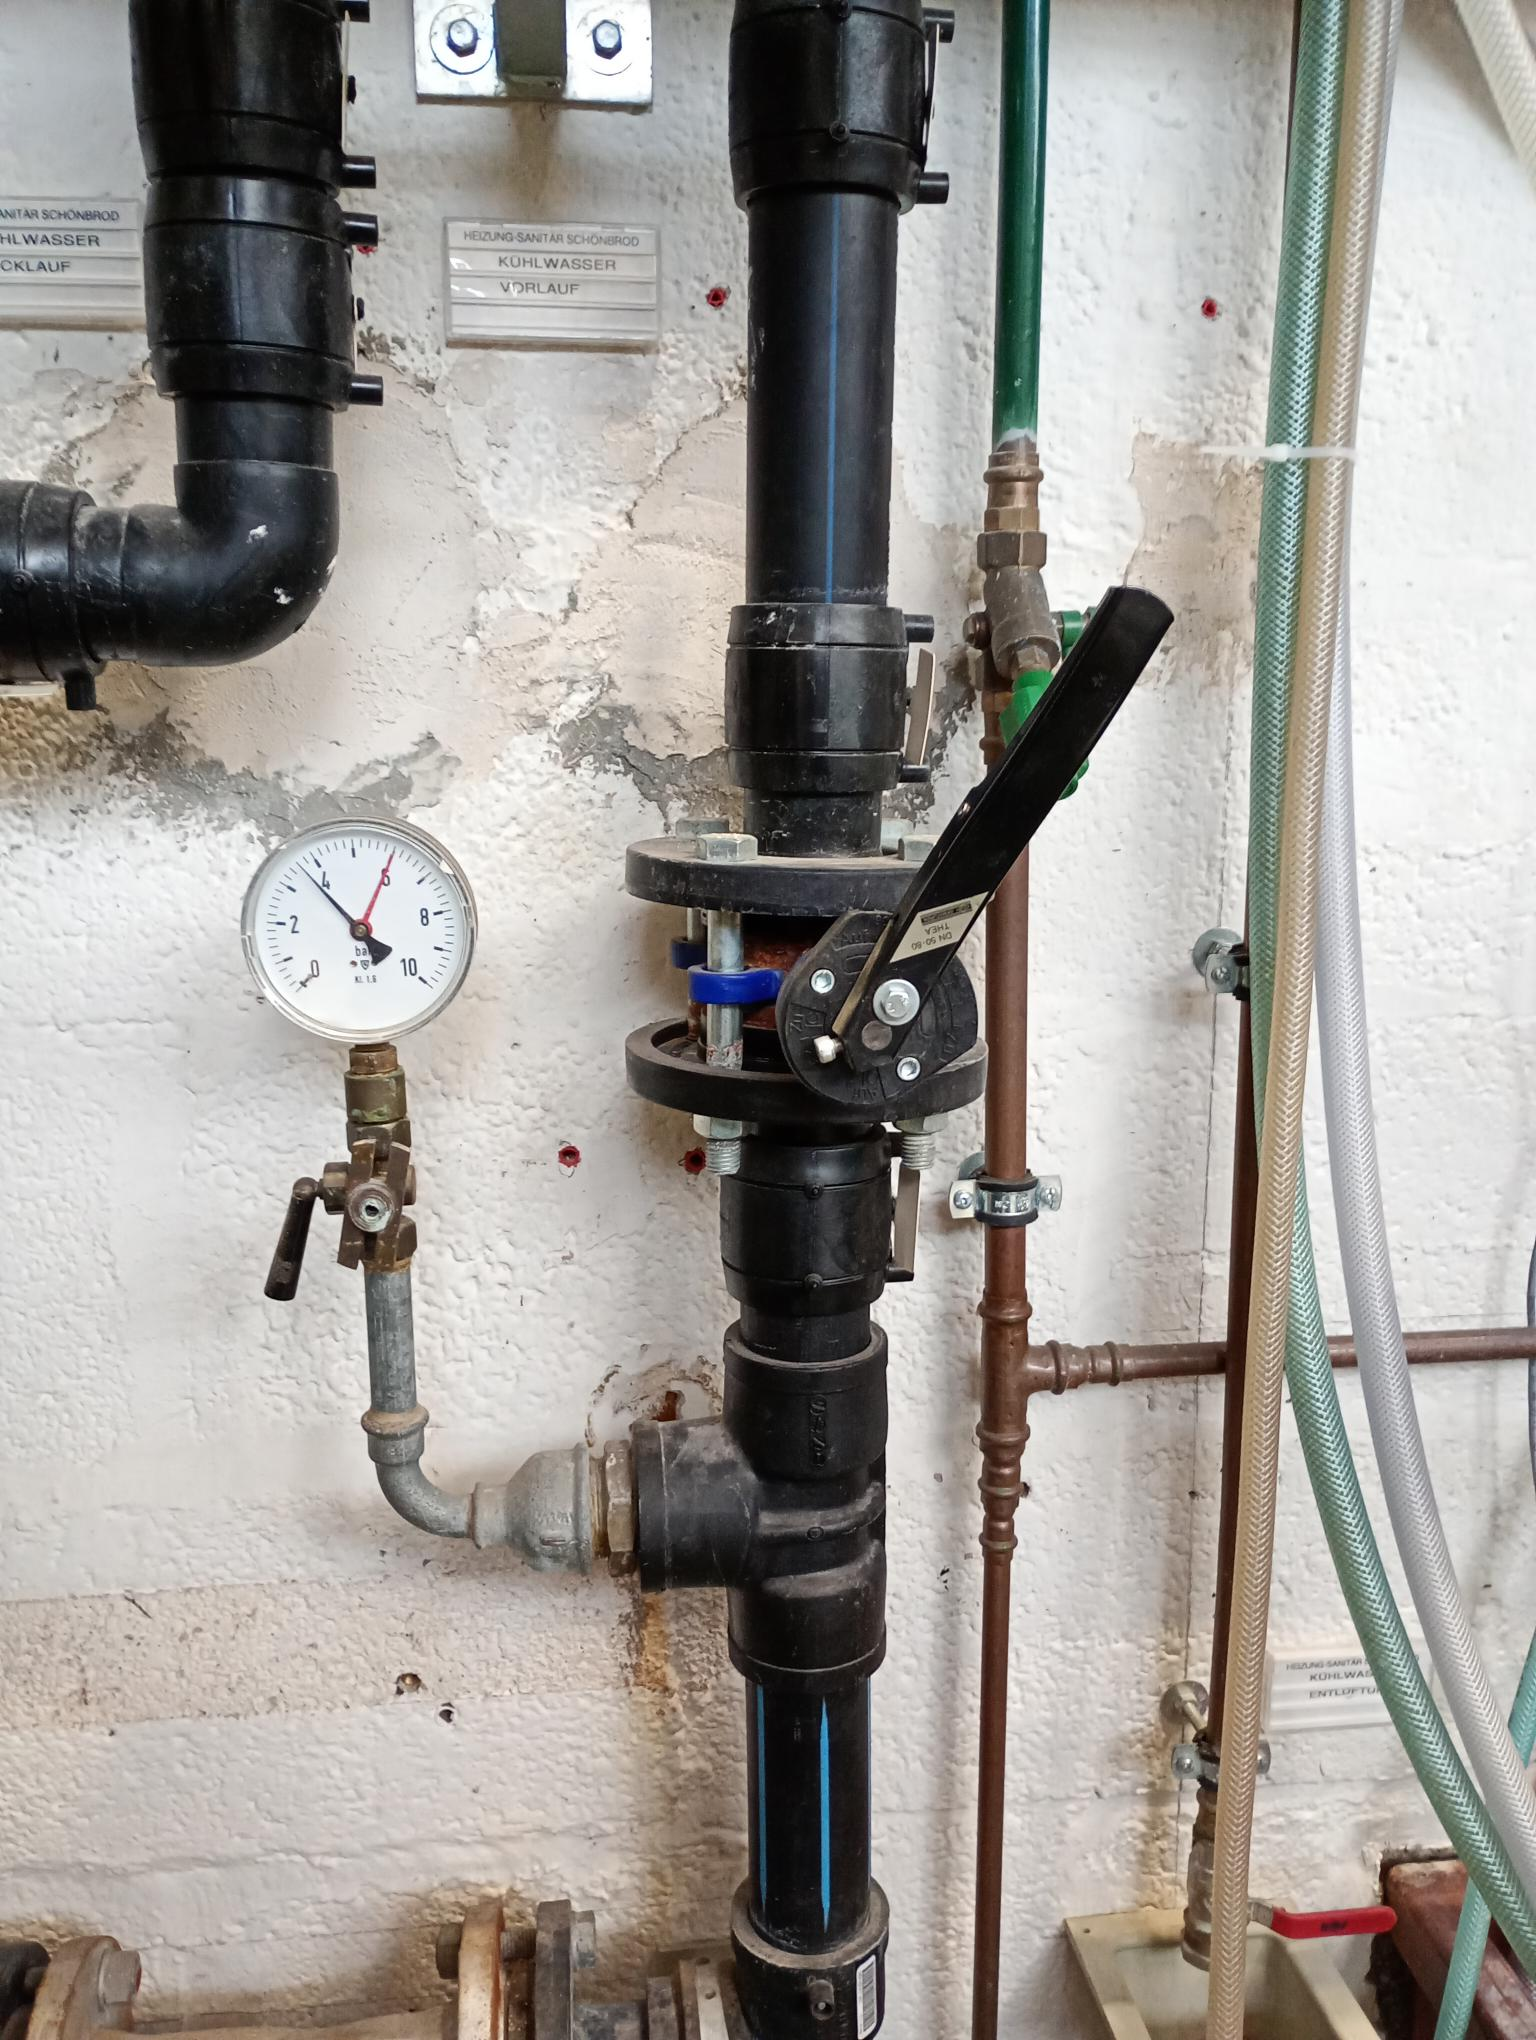
\includegraphics[height=8cm]{Cool5}
	\captionsetup{width=0.8\textwidth}
	\captionof{figure}{Cooling systems with \textbf{1.}Cooling for EC source and window \textbf{2.}Cooling for turbopump \textbf{3.}Not in use \textbf{4.}Main valve for cooling of the coils}
	\label{Cool2}
\end{figure}

\newpage

For safe operation, the electrical resistance of the cooling water has to be high enough to avoid that the coil current flows through the cooling water. This can be checked on the conductance meter (Leitwertmesser) (Figure \ref{Cool9}).\\

\textcolor{red}{\textbf{Check the electrical resistance of the cooling water (Figure \ref{Cool9}) bottom).}}\\

\begin{minipage}{.58\textwidth}

If the indicator is below $ 2\ \mu S/cm$ or $0.5\ M\Omega /cm$, the distillatory pump has to be activated for some time ($\pm 1$ hour), reducing the conductivity of the water. It can be activated in the section Rectifier MF on the `\textit{Magnetic Field}' tab in the Control System (Figure \ref{Cool10}). This will reduce the conductivity of the water. \\

	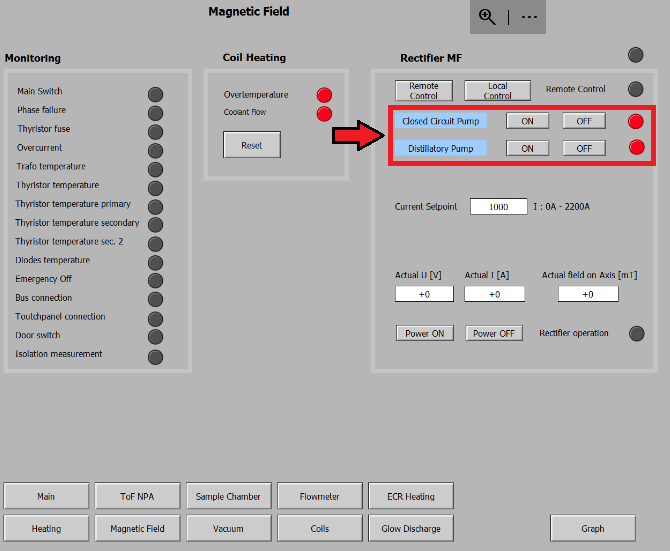
\includegraphics[width=\linewidth]{Cool10}
	\captionof{figure}{The `\textit{Magnetic Field}' tab in the Control System}
	\label{Cool10}
\end{minipage}
\begin{minipage}{.02\textwidth}
	$\ $\\
\end{minipage}
\begin{minipage}{.4\textwidth}


	\includegraphics[width=0.97\linewidth]{Cool9}
	\captionsetup{width=0.75\textwidth}
	\captionof{figure}{Closed water circuit pump with power switch (right) and conductance meter (bottom)}
	\label{Cool9}
\end{minipage}
\vspace*{0.5cm}

\begin{minipage}{.3\textwidth}
The cooling system for the cooling of the coils can be activated in the section Rectifier MF on the `\textit{Magnetic Field}' tab in the Control System (Figure \ref{Cool10}).\\

\textcolor{red}{\textbf{Activate the Closed Circuit Pump.}}\\
	
You can verify the coil temperature on the \textit{`Overview Coils'} tab in the Control System (Figure \ref{Coil}). The status of both pumps is also visible here, as is the status of the coolant Flow. Temperatures above $40^\circ C$ should be avoided.\\

All cooling systems are now ready.\\

In the future, the coils cooling will be activated automatically when the current in the coils is activated in the Control System.
	 
\end{minipage}
\begin{minipage}{.02\textwidth}
$\ $\\
\end{minipage}
\begin{minipage}{.68\textwidth}
\centering
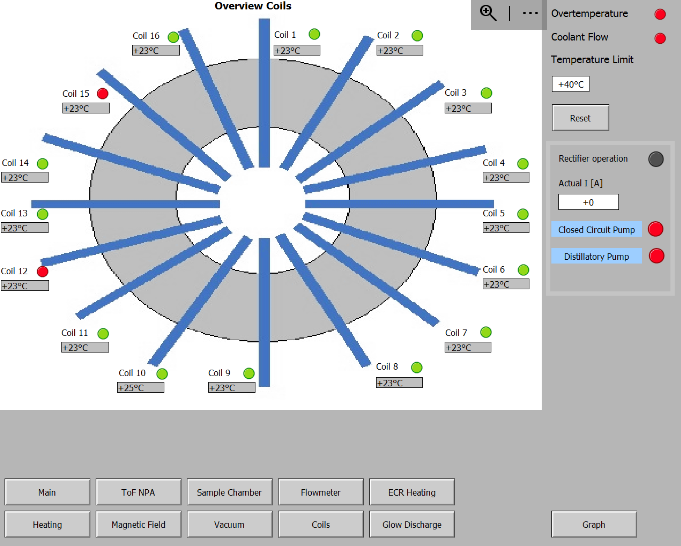
\includegraphics[width=0.98\linewidth]{Coil}
\captionsetup{width=0.75\textwidth}
\captionof{figure}{The \textit{`Overview Coils'} tab in the Control System}
\label{Coil}
\end{minipage}





\begin{minipage}{.68\textwidth}
\subsection{Magnetic field}
	
To activate the magnetic field, the cooling of the coils should be activated. You can initiate the coil current at the Magnetic field power supply (Figure \ref{Coil1}).\\

\textcolor{red}{\textbf{Remove the lock from the black lever arm of the magnetic field power supply. Turn the lever arm counter-clockwise to the position “ON”.}}\\

You can find the key of the lock inside one of the drawers of the main TOMAS computer table.\\

When the magnetic field power supply is "ON", the green `STANDBY' LED is activated. When the red LED `STÖRUNG' is activated, you can push the reset button (F8 on Figure \ref{Coil2}). When the red LED keeps activated, there is a problem with the power supply. Turn the lever arm clockwise to the position “OFF” and call for specialized help.\\


\textcolor{red}{\textbf{Set a value for the coils current and press “DC ON”. }}\\
	
When the coils current is activated, the white LED `DC-EIN' is activated. Verify that the value $A_{set}$ equals  $A_{act}$.\\
	
\end{minipage}
\begin{minipage}{.02\textwidth}
	$\ $\\
\end{minipage}
\begin{minipage}{.3\textwidth}
\centering
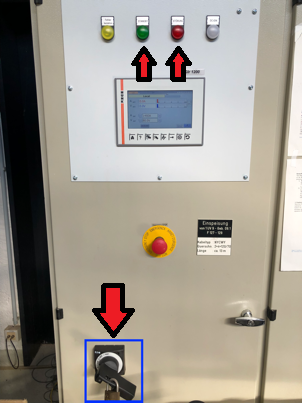
\includegraphics[width=0.98\linewidth]{Coil1}
\captionsetup{width=0.75\textwidth}
\captionof{figure}{The magnetic field power supply}
\label{Coil2}
\end{minipage}



\begin{minipage}{.48\textwidth}
The value of the current can vary (theoretically) between 0 A and 2200 A. Note that for EC operation, the position of the EC resonance layer depends on the magnetic field.  An overview of the position of the EC resonance layer as function of the coil current is given in Figure \ref{ECR} for the fundamental frequency. For second harmonic heating, the coil current should be halved.\\

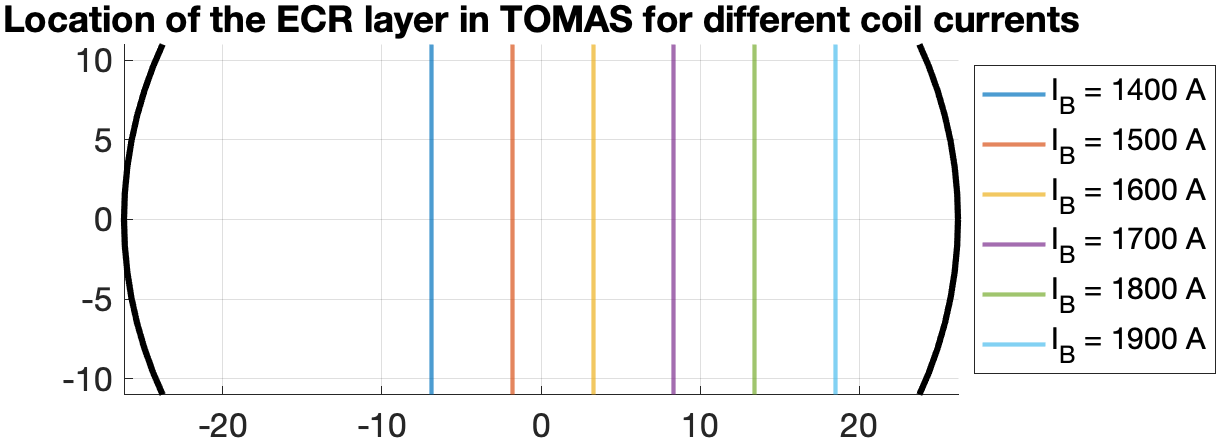
\includegraphics[width=0.98\linewidth]{ECR}
\captionsetup{width=0.75\textwidth}
\captionof{figure}{The magnetic field power supply touchscreen}
\label{ECR}

\end{minipage}
\begin{minipage}{.02\textwidth}
$\ $\\
\end{minipage}
\begin{minipage}{.5\textwidth}
\centering
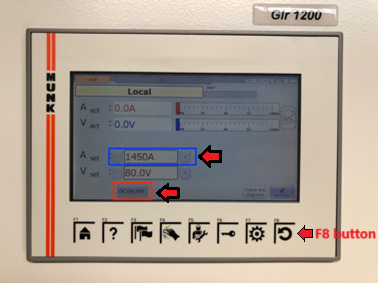
\includegraphics[width=0.98\linewidth]{Coil2}
\captionsetup{width=0.75\textwidth}
\captionof{figure}{The magnetic field power supply touchscreen}
\label{Coil1}
\end{minipage}



\begin{center}
	\textcolor{red}{\textbf{Note! Don’t use the magnetic field during Glow Discharge operation!}}\\
\end{center}
\vspace{0.2cm}


\begin{minipage}{.63\textwidth}

\subsection{EC operation}


EC operation is controlled remotely by the Operator PC. The EC amplifier has to be activated manually.\\

\textcolor{red}{\textbf{Activate the EC by pulling the black lever upwards (Figure \ref{EC1}).}}\\

Wait until the amplifier is ready. This is indicated by LED number 2 on Figure \ref{EC1} (START/STOP PREHEAT/READY). The LED for remote operation should also be activated (LED number 1 on Figure \ref{EC1}).\\

When EC is on, the first display shows the forwarded power, the second one shows the reflected power. To maximize the power absorbed by the plasma, the EC system should be matched (see section \ref{}).\\

The EC amplifier is now ready for operation. 

	
\end{minipage}
\begin{minipage}{.02\textwidth}
	$\ $\\
\end{minipage}
\begin{minipage}{.35\textwidth}
\centering
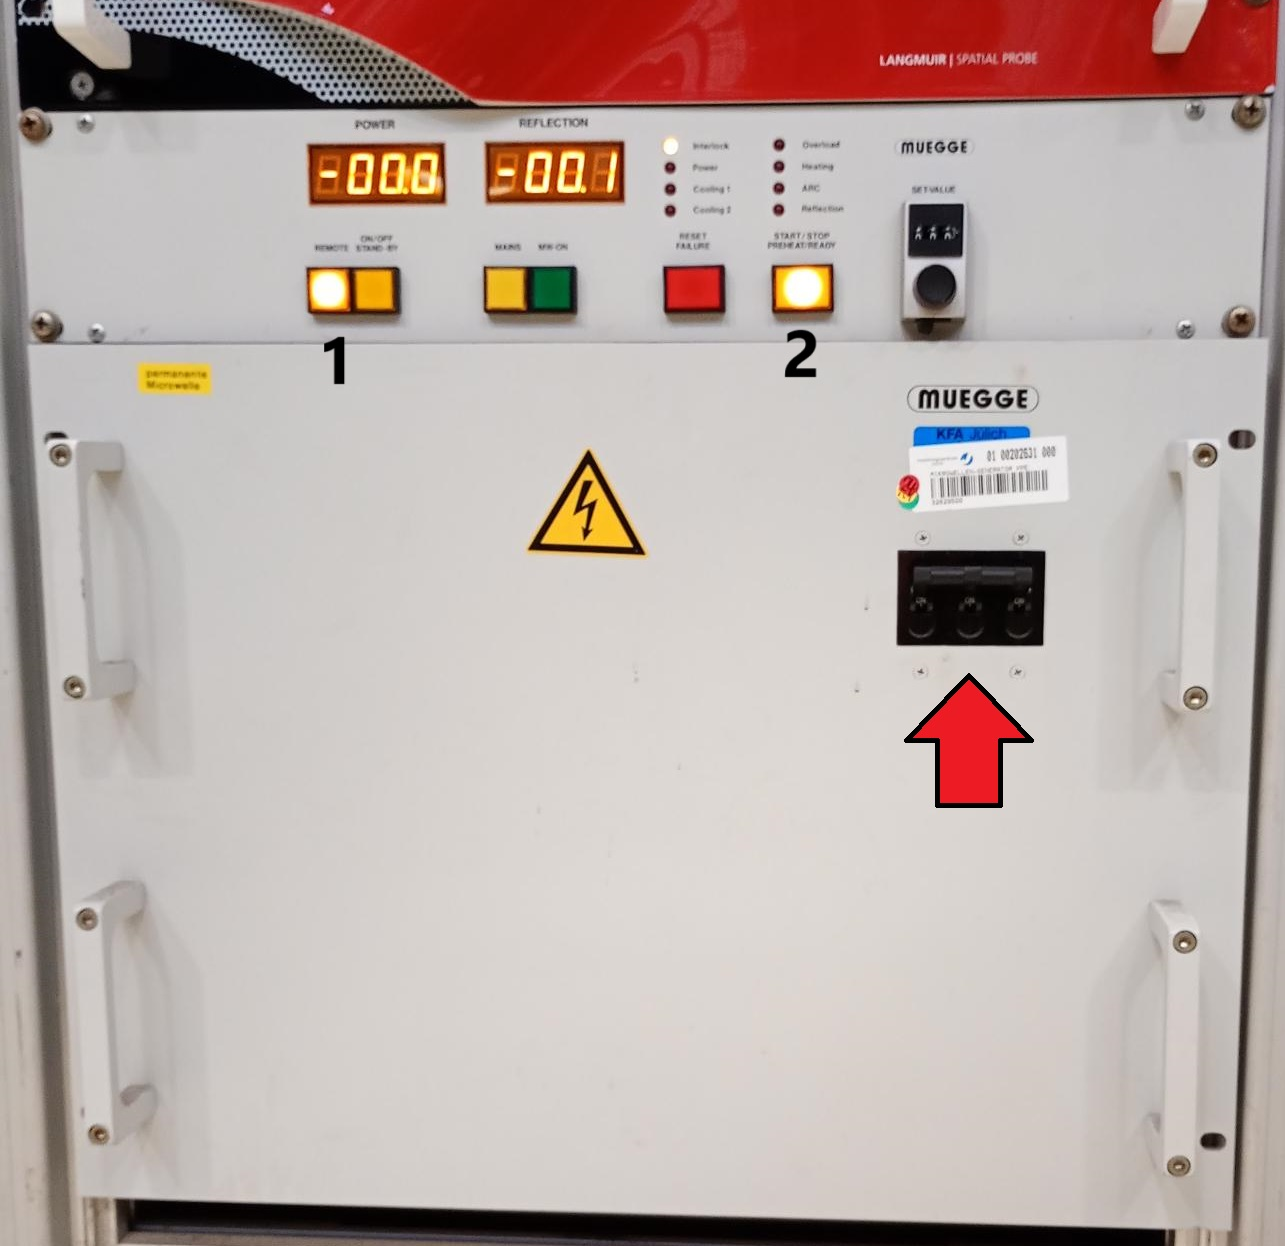
\includegraphics[width=\linewidth]{EC1}
\captionsetup{width=0.75\textwidth}
\captionof{figure}{The EC amplifier}
\label{EC1}
\end{minipage}





\newpage
\subsection{IC operation}




\newpage	
%%%%%%%%%%%%%%%%%%%%%%%%%%%%%%%%%%
\section{Operational procedures}%%	
%%%%%%%%%%%%%%%%%%%%%%%%%%%%%%%%%%


\subsection{EC matching procedure}


\subsection{IC matching procedure}




%The wave equation can be written as:
%\begin{equation}
%\left[ \left( \omega^2 - c^2 k^2\right)  \matr{e} + c^2 \vec{k}\cdot \vec{k}\right] \cdot \vec{E_1}= \dfrac{1}{\epsilon_0} i\omega \vec{J_1}
%\end{equation}
%To find a solution $\vec{E_1}(\vec{r},t)$ for this wave equation (dispersion relation) we need to eliminate $\vec{J_1}$. Taking into account possible boundary conditions, we can find a relation between $\vec{J_1}$ and $\vec{E_1}$ : $\vec{J_1} = \matr{\sigma}\cdot\vec{E_1}$, where $\matr{\sigma}$ is the conductivity tensor.\\
%
%For a cold electron plasma, where there is no acoustic coupling and collisions with ions are neglected, we find: $i\omega \vec{J_1}=\epsilon_0\omega^2_p\vec{E_1}$ with the plasma frequency $\omega^2_{pe} = n_eq^2_e/m_e\epsilon_0$ . The quantity $\epsilon_0\omega^2_p/i\omega$ plays the role of complex conductivity. The wave equation reduces to:
%\begin{equation} \left[ \left( \omega^2 - c^2 k^2-\omega^2_p\right)   \matr{e} + c^2 \vec{k}\cdot \vec{k}\right] \cdot \vec{E_1}= \vec{0}\end{equation}
%
%A wave is longitudinal if $\vec{E_1} \parallel \vec{k}$. This wave is always electrostatic. There is no oscillating magnetic field since $\vec{k} \times \vec{E_1}=\omega \vec{B_1}=\vec{0}$. Since $ \vec{k}\cdot \vec{k} \cdot \vec{E_1}=k^2\vec{E_1}$, the dispersion relation reduces to $\omega^2=\omega^2_{pe}$. These are the well-known local plasma oscillations that do not propagate in the plasma.\\
%
%A wave is transversal if $\vec{E_1} \perp \vec{k}$. With $\vec{E_1}$ a vector $\vec{B_1}$ is associated:  $\vec{k} \times \vec{E_1}=\omega \vec{B_1}$. This wave is always electromagnetic, since with the oscillating electric field an oscillating magnetic field is associated with amplitude $B_1=kE_1/\omega$. Since $ \vec{k}\cdot \vec{k} \cdot \vec{E_1}=\vec{0}$, the dispersion relation becomes $\omega^2=c^2k^2+\omega^2_{pe}$.\\
%
%The plasma is dispersive and has a refractive index and a dielectric constant: $n^2=c^2k^2/\omega^2=\epsilon_r=1-\omega^2_{pe}/\omega^2$.
%\begin{itemize}
%	\item With $\omega < \omega_{pe}$ correspond imaginary values of $k$ and there is no wave propagation $(n<0)$.
%	\item With $\omega = \omega_{pe}$ corresponds a cut-off.
%	\item For $\omega > \omega_{pe}$, real values of $k$ exist and the wave can propagate undamped through the plasma.
%\end{itemize}
%
%As a wave propagates into a plasma several different phenomena can occur with respect to the deposition of its wave energy: reflection, transmission, absorption and mode conversion. An incident wave is in general partially reflected and partially transmitted.\\

%\textbf{Reflection} For an outside launch the wave sees an increasing density as it propagates towards the centre. It also sees a slightly increasing magnetic field because of the $1/R$ dependence. As it reaches a zone where it cannot propagate, the wave reflects back. At this point $k\rightarrow0, n\rightarrow0$ and we reach a cut-off.\\
%
%\textbf{Transmission} If the evanescent region is small (with respect to the wavelength) the wave can partially tunnel through this region.\\
%
%\textbf{Absorption} A strong wave-particle resonance can occur leading to a strong absorption. This is the case where $k\rightarrow\infty$. The resonance occurs when the parallel Doppler shifted frequency is equal to an exact harmonic of the cyclotron frequency: $\omega = k_\parallel v_\parallel+\ell \omega_{ce}$. 
%\begin{itemize}
%	\item $\ell=0$: Landau damping
%	\item $\ell=0$: Fundamental frequency heating
%	\item $\ell=0$: Second harmonic heating
%\end{itemize}
%
%\textbf{Mode conversion} This involves two different plasma waves. the wave encounters a wave resonance which mode converts it into a different type of plasma wave. Again $k\rightarrow\infty$. Some of the energy of the incident wave is transferred to the second wave which propagates further into the plasma.\\
%
%In a magnetized plasma the Lorentz force also acts on the charge carriers. We neglect electron-ion collisions and the acoustic coupling. The presence of an external magnetic field $\vec{B_0}$ introduces an electron cyclotron frequency $\omega_{ce} = -q_eB_0/m_e$. This magneto-plasma behaves as a circularly birefringent medium. We obtain two dispersion relations and two different waves can be distinguished. 
%
%\begin{itemize}
%	\item \textbf{Ordinary wave} (O-wave) or L-circularly polarized wave.
%		\begin{equation}
%		\omega^2=c^2k^2+\dfrac{\omega^2_{pe}\omega}{\omega + \omega_{ce}}
%		\end{equation}
%	\item \textbf{Extraordinary wave} (X-wave) or R-circularly polarized wave.
%		\begin{equation}
%		\omega^2=c^2k^2+\dfrac{\omega^2_{pe}\omega}{\omega - \omega_{ce}}
%		\end{equation}
%\end{itemize}
%
%\newpage

%




\end{document}